% Please use the skeleton file you have received in the
% invitation-to-submit email, where your data are already
% filled in. Otherwise please make sure you insert your
% data according to the instructions in PoSauthmanual.pdf
\documentclass{PoS}
\usepackage{tikz}
\usepackage{placeins}
\usepackage{wrapfig}
\usepackage{appendix}
\usepackage{todonotes}
\usepackage{comment}
\usetikzlibrary{arrows.meta}

\title{A Comparison between a Novel Algorithm for Finite Differences and the Established Finite Element Method to Simple Electrostatic Potentials}

\ShortTitle{Electrostatics: an Approach using Finite Differences and Finite Element}

\author{\speaker{Hayden P. Scholz}\\
        Tufts University, USA\\
        E-mail: \email{hayden.scholz@tufts.edu}}
\author{\speaker{J. Emmanuel Flores}\\
        Tufts University, USA\\
        E-mail: \email{jflore10@tufts.edu}}
        
\author{\speaker{Cullen M. Sullivan}\\
        Tufts University, USA\\
        E-mail: \email{cullen.sullivan@tufts.edu}}

\abstract{
We present two different methods for numerically solving Poisson’s equation. We develop a novel General Finite Differences Method (GFDM) that uses a graph data structure to represent an arbitrary mesh layout. With an arbitrary graph structure for its mesh, the method is anticipated to work well for irregular geometries. The method is compared to the more efficient and more complex Finite Element Method (FEM), which is implemented using the well-established and widely used FEniCS software. The comparison is made using the two-dimensional coaxial cable problem, which is analytically solvable, well-understood, and widely applicable. We study ideal hyper-parameters of the general finite differences method for the coaxial problem and find the solution is slightly noisy and sensitive to relative placements of nodes of the mesh. These errors grow smaller and converge to the analytical solution for increasing node counts, and the ideal neighbors per node is six. We find the GFDM is less complex to implement for complex geometries than the FEM and generates a good approximate solution with slightly more error. We look forward to testing the GFDM on irregular geometries in the near future.
}

\FullConference{Classical Electromagnetism Theory I (PHY\-0145)\\
		December, 2023\\
		Tufts University, Medford, MA}



\begin{document}

\section{Introduction: Physics and the need for Numerical Methods}
% \subsection{Physics and the need for Numerical Methods}
It is common in the physical sciences to face problems expressed as differential equations. Often, these models are complex, and their analytical solution is either complicated, or does not exist. Therefore, there exists the need to develop alternative tools to attack the differential models in question. A common approach is a numerical approach. The basic idea of numerical methods is to transform a differential problem into a discrete form to reduce the degrees of freedom of the problem to a finite quantity. This is not straightforward, and there are many ways to discretize such equations, both spatially and temporally. One of the most popular methods is the finite difference method (FDM) for its direct and easy-to-implement approach. Derivatives are replaced by quotients, and the respective differential operators are replaced by their discrete counterparts which results in a set of algebraic equations that can be readily solved. In this work we will focus on two numerical schemes. We develop a new scheme of FDM with the incorporation of the graph data structure. Then, we will focus on the finite element method (FEM), which, in recent years, has become very popular and widely used by the community. Finally, we make a comparison between the results of the established FEM and our newly developed FDM.

\section{Laplace and Poisson Equation}
Partial differential equations (PDEs) are classically divided into three main types based on their geometric and physical interpretations: hyperbolic, parabolic, and elliptic. Hyperbolic PDEs govern wave phenomena and information propagation with finite speed, on the other hand parabolic PDEs model diffusion processes where information spreads gradually and continuously over time, like heat flow, and finally, elliptic PDEs describe equilibrium states or systems that tend to smooth out disturbances. The wave equation, diffusion equation, and Poisson's equation serve as prominent examples of these respective types. For further exploration, \cite{nandakumaran2020partial} provides a comprehensive introduction. However, our focus is a class of situations in which these equations can appear, namely, electrostatic theory.
% These equations appear in a variety of physical problems and mathematically represent the standard class of elliptic partial differential equations (PDEs). It's also important to note that some numerical schemes for complicated PDEs are based on Poisson's equation. 

Electrostatic Theory describes the physical phenomena of electric charges in the situation where all the sources of charge are kept stationary. In electrostatics, the force between electric charges is given as a central force defined by Coulomb’s Law. The influence that a distribution of charges has on a test charge placed anywhere in space is described by a vector field called the electric field. Since the electric field is generated by a central force, the curl of the electric field will always be zero. By Helmholtz's Theorem, any curl-less vector field can be represented as the gradient of a scalar function;  thus, the electric field $\mathbf{E}$ is defined as the negative gradient of the scalar potential $V$, so
\begin{equation}
    \mathbf{E} = -\nabla V.
\end{equation}
Furthermore, since the E-field is defined by a charge distribution, these definitions can be combined into one equation relating the electric potential and charge distribution, $\rho$, namely, Poisson’s equation, which is given by 
\begin{equation}
    \nabla^2 V = -\frac{\rho}{\epsilon_0}.
\end{equation}
In regions where there is no net charge distribution, this reduces to Laplace’s equation, which is given by 
\begin{equation}
    \nabla^2 V = 0.
\end{equation}

For a unique solution of Poisson’s equation, there must be some specified boundary conditions which are complete over the whole boundary. There are three different types of boundary conditions; 1. Dirichlet, where the potential is specified on the whole boundary, 2. Neumann, where the normal component of the gradient of the potential is specified on the entire boundary, and 3. Mixed, where the potential is specified over a portion of the boundary and the gradient of the potential is specified on the remainder of the boundary. 

\newpage
\section{Finite Differences and Finite Element Methods}

\subsection{Finite Differences Method}
The FDM generates a discrete (usually Cartesian) spatial grid (mesh) of solution nodes then projects boundary conditions onto the mesh. The differential model is approximated to quotients, and linear equations are generated to describe local relations interior to the mesh. A high performance linear algebra package can be used to solve the linear equations to find the best allowed solution to the differential equation. Although the approximate solution converges for sufficiently small mesh spacing, the Cartesian grid can converge prohibitively slowly for non-rectangular geometries \cite{Landau2015}.

For solving Poisson's Equations for irregular geometries, we have developed an expansion of the FDM to avoid use of a strictly Cartesian grid. We present the General Finite Differences Method (GFDM) which instead uses an arbitrary mesh represented as a graph data structure. The GFDM accepts Dirichlet boundary conditions and generates a mesh to respect the geometry of the system. The method has been described in literature \cite{PERRONE197545} \cite{KAMYABI2019233}, and we have implemented the mathematics (\ref{sec:gfdm_math}) and algorithm to be as simple to use as possible.

\subsection{The General Finite Differences Method Algorithm}
\begin{wrapfigure}{R}{0.30\linewidth}
    \centering
    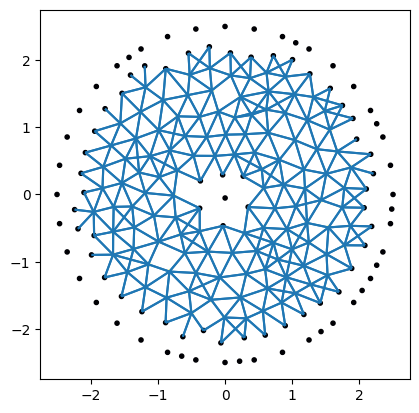
\includegraphics[width=0.9\linewidth]{Figures/GFDM/Coax_GFDM_Connectivity.png}
    \caption{Sample connectivity graph for the GDFM (124 nodes, 6 target neighbors). Black nodes are boundary nodes. Intersections of lines are nodes where potential will be solved using information from its neighbors.}
    \label{fig:coax_gfdm_connectivity}
\end{wrapfigure}
We give an overview of the GFDM algorithm. First, the user provides a collection of points that define some 2D boundary (no holes) and a function declaring arbitrary Dirichlet boundary conditions. The solver generates an irregular mesh within the boundary. The meshing is deterministic and generates nodes such that nearby nodes are not separated by more than some maximum edge length. The mesher \cite{Schlomer_pygalmesh_Python_interface} places nodes where they are needed to describe the space. Next, for each non-boundary node, the solver selects a few nearby points to make neighbors of that node. Figure \ref{fig:coax_gfdm_connectivity} shows a sample output of the entire connectivity step. This is the slowest step and runs at $O(n^2)$. Having built the connectivity graph, an $n \times n$ ($n$ is the number of nodes in the mesh) matrix is built with elements as defined by Equation \ref{eq:gfdm_matrix_elements} using information from neighbor nodes. The matrix is a linear system of $n$ equations that, when solved, directly supply numerical solutions for potentials at every node in the mesh. By only considering interactions between nearby nodes, the potential of each node only depends on a few others, keeping the solution matrix sparse. Various packages were invaluable, including those for managing the graph data structure \cite{networkx}, plotting \cite{matplotlib}, and numerical algorithms \cite{numpy}.

\subsection{Finite Element Method}

FEM is a numerical technique used to find approximate solutions to problems governed by partial differential equations such as Poisson's or Laplace's equation. The main idea is to break down the domain where the problem is defined, which can be highly complex, into smaller and simpler parts called elements. The method analyzes each element separately by considering how it interacts with its neighboring elements. Elements can be regarded as a basis set.

The goal of the method is to represent the overall system mathematically by assembling the behavior of these individual elements. By doing this for all elements and considering all their interactions, the method provides an approximation of the system's behavior. This approach allow us to study and simulate various physical phenomena, such as stress, heat transfer, fluid flow, and electromagnetic phenomena in a computationally efficient manner.

\section{Simulated Problem: Coaxial Cable}

% \subsection{Coaxial Cable}
\begin{wrapfigure}[12]{R}{0.30\linewidth}
\centering
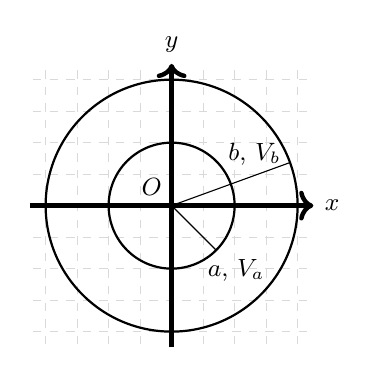
\begin{tikzpicture} [scale=0.40]    
\draw[help lines, color=gray!30, dashed] (-4.4,-4.4) grid (4.4,4.4);
\draw[->,ultra thick] (-4.5,0)--(4.5,0) node[right]{\small $x$};
\draw[->,ultra thick] (0,-4.5)--(0,4.5) node[above]{\small $y$};
\draw [thick] circle [radius=2.0];
\draw [thick] (0,0) circle [radius=4];
\draw[-, rotate around={-45:(0,0)}] (0,0) -- (2,0)  node [pos=1.45] {\small $a$, $V_a$};
\draw[-, rotate around={20:(0,0)}] (0,0) -- (4.,0) node [pos=0.7, above] {\small $b$, $V_b$};
\draw[fill=black](0,0) circle (1 pt) node [anchor=south east] {\small $O$};
\end{tikzpicture}
\caption{2-dimensional schematic projection of the coaxial problem.}
\end{wrapfigure}
As the main example, let's solve the problem of the coaxial cable, which is shown in the following diagram, and in which we have two concentric cylinders, one with radius $r=a$ and the other with $r=b$, where $a<b$ and in this radius, the potential is given by $V_a$ in $a$ and $V_b$ in $b$. 
We write the problem using cylindrical coordinates, so Laplace's equation is given by 
\begin{equation}
    \nabla^2 V = \frac{1}{r}\frac{\partial}{\partial r}\left(r\frac{\partial V}{\partial r}\right) + \frac{1}{r^2}\frac{\partial^2 V}{\partial \theta^2} + \frac{\partial^2 V}{\partial z^2} = 0,
\end{equation}
By rotational invariance, we assert the potential has no angular part. Because we're also assuming that the length of the coaxial cable is large compared to the radius of the cylinder, we collapse the problem onto two dimensions. By ignoring $z$ dependence, we use the following differential equation with a solution
\begin{equation}
    \frac{1}{r}\frac{\partial}{\partial r}\left(r\frac{\partial V}{\partial r}\right)=0 \rightarrow V(r) = \beta + \alpha\ln\left(r\right).
\end{equation}
% which can be easily integrated to give the general solution 
% \begin{equation}
%     u(r) = \beta + \alpha\ln\left(r\right), 
% \end{equation}
If we use the Dirichlet boundary conditions, we can express the solution for the potential and the electric field, as follows 
\begin{equation}
    V(r) = \frac{V_b - V_a}{\ln(b/a)}\ln\left(\frac{r}{a}\right) + V_a, \rightarrow \mathbf{E} = \frac{V_a - V_b}{\ln(b/a)}\frac{1}{r}\hat{\mathbf{r}}.
    \label{eq:coax_pot}
\end{equation}
% We can calculate the electric field, which is given by 

% \begin{equation}
%     \mathbf{E} = \frac{u_a - u_b}{\ln(b/a)}\frac{1}{r}\hat{\mathbf{r}}.
% \end{equation}

\section{Results}
\subsection{General Finite Differences Method}
\begin{figure}[hbt]
\begin{minipage}{0.32\linewidth}
    \centering
    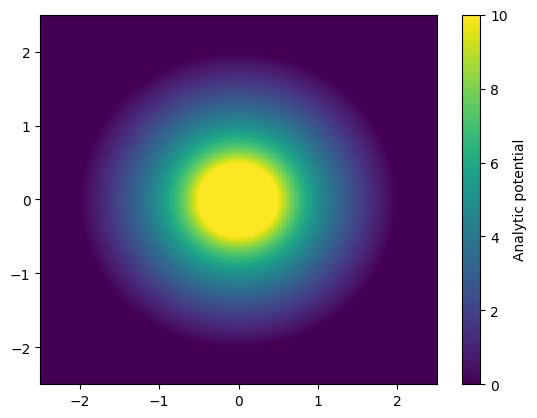
\includegraphics[width=\linewidth]{Figures/GFDM/Coax_Analytic.png}
\end{minipage}
\hfill
\begin{minipage}{0.32\linewidth}
    \centering
    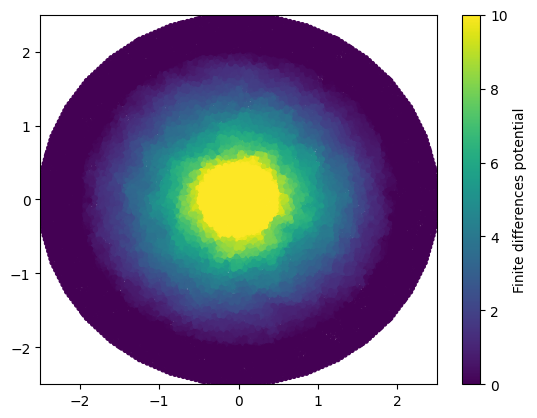
\includegraphics[width=\linewidth]{Figures/GFDM/Coax_GFDM.png}
\end{minipage}
\hfill
\begin{minipage}{0.32\linewidth}
    \centering
    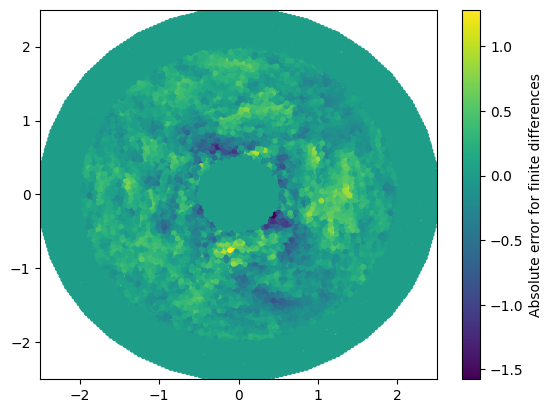
\includegraphics[width=\linewidth]{Figures/GFDM/Coax_GFDM_Error.png}
\end{minipage}
\caption{Left: Analytic solution to the two dimensional coaxial problem (Equation \ref{eq:coax_pot}). Center: GFDM solution to the coaxial problem with 10101 nodes and 6 target neighbors per node. Right: Absolute error per node for the GFDM solution (numerical - analytical). RMS error = 0.205}
\label{fig:gfdm_coax_solutions}
\end{figure}

\begin{wrapfigure}{R}{0.45\linewidth}
    \centering
    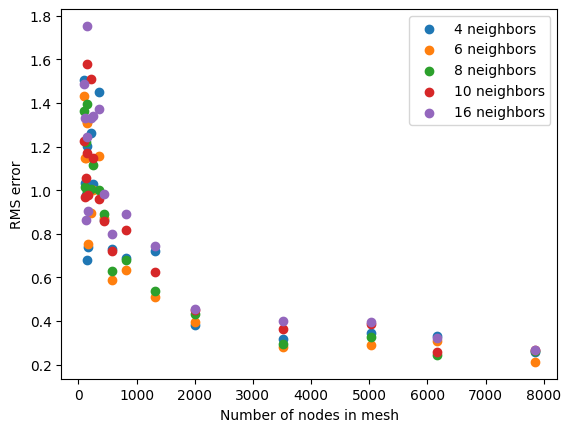
\includegraphics[width=\linewidth]{Figures/GFDM/Coax_GFDM_Nodes_Neighbors_RMS.png}
    \caption{RMS error for independent GFDM solutions of the coaxial problem.}
    \label{fig:gfdm_coax_nodes_neighbors}
\end{wrapfigure}
We implemented the GFDM method and applied boundary conditions to numerically solve the coaxial cable problem. The inner conductor has radius 0.5 and is set to 10 V. The outer conductor has radius 2.0 and is grounded. Figure \ref{fig:gfdm_coax_solutions} has the analytic solution, the GFDM numerical solution, and the error (in units of potential) of the method. The GFDM method outputs a reasonable solution but notably does not retain perfect spherical isotropy. This is to be expected because mesh generation does not require any form of spatial symmetry.

We probe how well the GFDM performs as a function of its hyper-parameters. We can control the density of nodes of the mesh and the target number of connections to nearby nodes that are formed (neighbors). Figure \ref{fig:gfdm_coax_solutions} summarizes the results of repeated independent solutions. We investigate root mean square (RMS) error between GFDM solutions and the analytic solution to probe the overall performance of the GFDM solver over the entire mesh. We find that RMS error decreases is lower for higher node count which is desired behavior. This suggests the method converges for large node counts, but for the coaxial problem, node counts above 10,000 cause prohibitively slow runtime and were not investigated. Investigation of solutions showed that higher node counts tended to produce solutions with regions of peak error with less severe error and of smaller area, but these solutions did not have fewer "hotspots" of high error.

Notably for low node counts, there is significant noise between outputs. This indicates that solutions for low node counts are sensitive to "choices" made by the meshing algorithm when selecting positions of nodes within the region to be solved. Small perturbations of relative node positions can cause unfavorable neighbor selections which cause non-negligible noisy errors in the solution. As the number of nodes increase, though, this effect is smoothed out, and noise between similar solutions because less prominent.

With this study, we compare the effect of how many neighbors are made per node on the goodness of solution, but we were surprised to find little effect of neighbor count on the goodness of solutions for high node counts. Upon close inspection for high number of nodes, we see that 16 neighbors typically performs worst. This makes sense because we think too many neighbors will make a node "too informed" about points that are too far away and harm the local intent of the algorithm. Also, we see that 6 neighbors typically performs best. 4 neighbors is too few and can cause asymmetric neighbor selection which can cause noisy error, but 6 neighbors is enough to make an overly asymmetric neighbor selection unlikely.

\subsection{Finite Element Method}

To facilitate a comprehensive comparison between FDM and FEM methodologies, we opted to simulate the same problem and juxtapose the outcomes. The potential details mirror those of the GFDM, underscoring the significance of delineating the specifics of the FEM approach. In our implementation, we employed the standard Lagrange family of elements as the foundation for the function space housing the solution. Furthermore, we selected a polynomial degree of 1, a well-established choice in the literature for addressing such problems. A nuanced yet crucial distinction from the GFDM lies in our approach: here, the solution is derived through interpolation between elements, providing a solution at every point within the defined mesh. Figure \ref{fig:VE_Fem} has the FEM solution to the coaxial problem. It is imperative to emphasize that, owing to the inherent workings of this methodology, we have successfully computed not only the potential field but also the electric potential. The latter is a conventional subject covered in standard textbooks on  theory. Finally, all the results were obtained using FEniCS, a powerful framework for solving PDEs using the FEM method \cite{alnaes2015fenics}, \cite{logg2012automated}.

\begin{figure}[hbt]
    \centering
    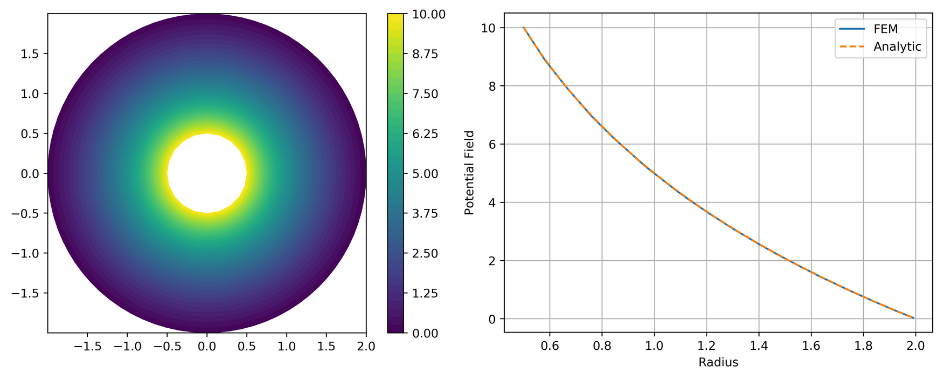
\includegraphics[width = 0.80\linewidth]{Figures/FEM/Pot_and Comparisson.png}
    \caption{Approximate solution to the two dimensional coaxial problem (Equation \ref{eq:coax_pot}). Right: Comparison between the analytical and approximate solution using FEM, RMS error = 0.008.}
    \label{fig:VE_Fem}
\end{figure}

\begin{comment}
\begin{wrapfigure}{R}{0.4\linewidth}
    \centering
    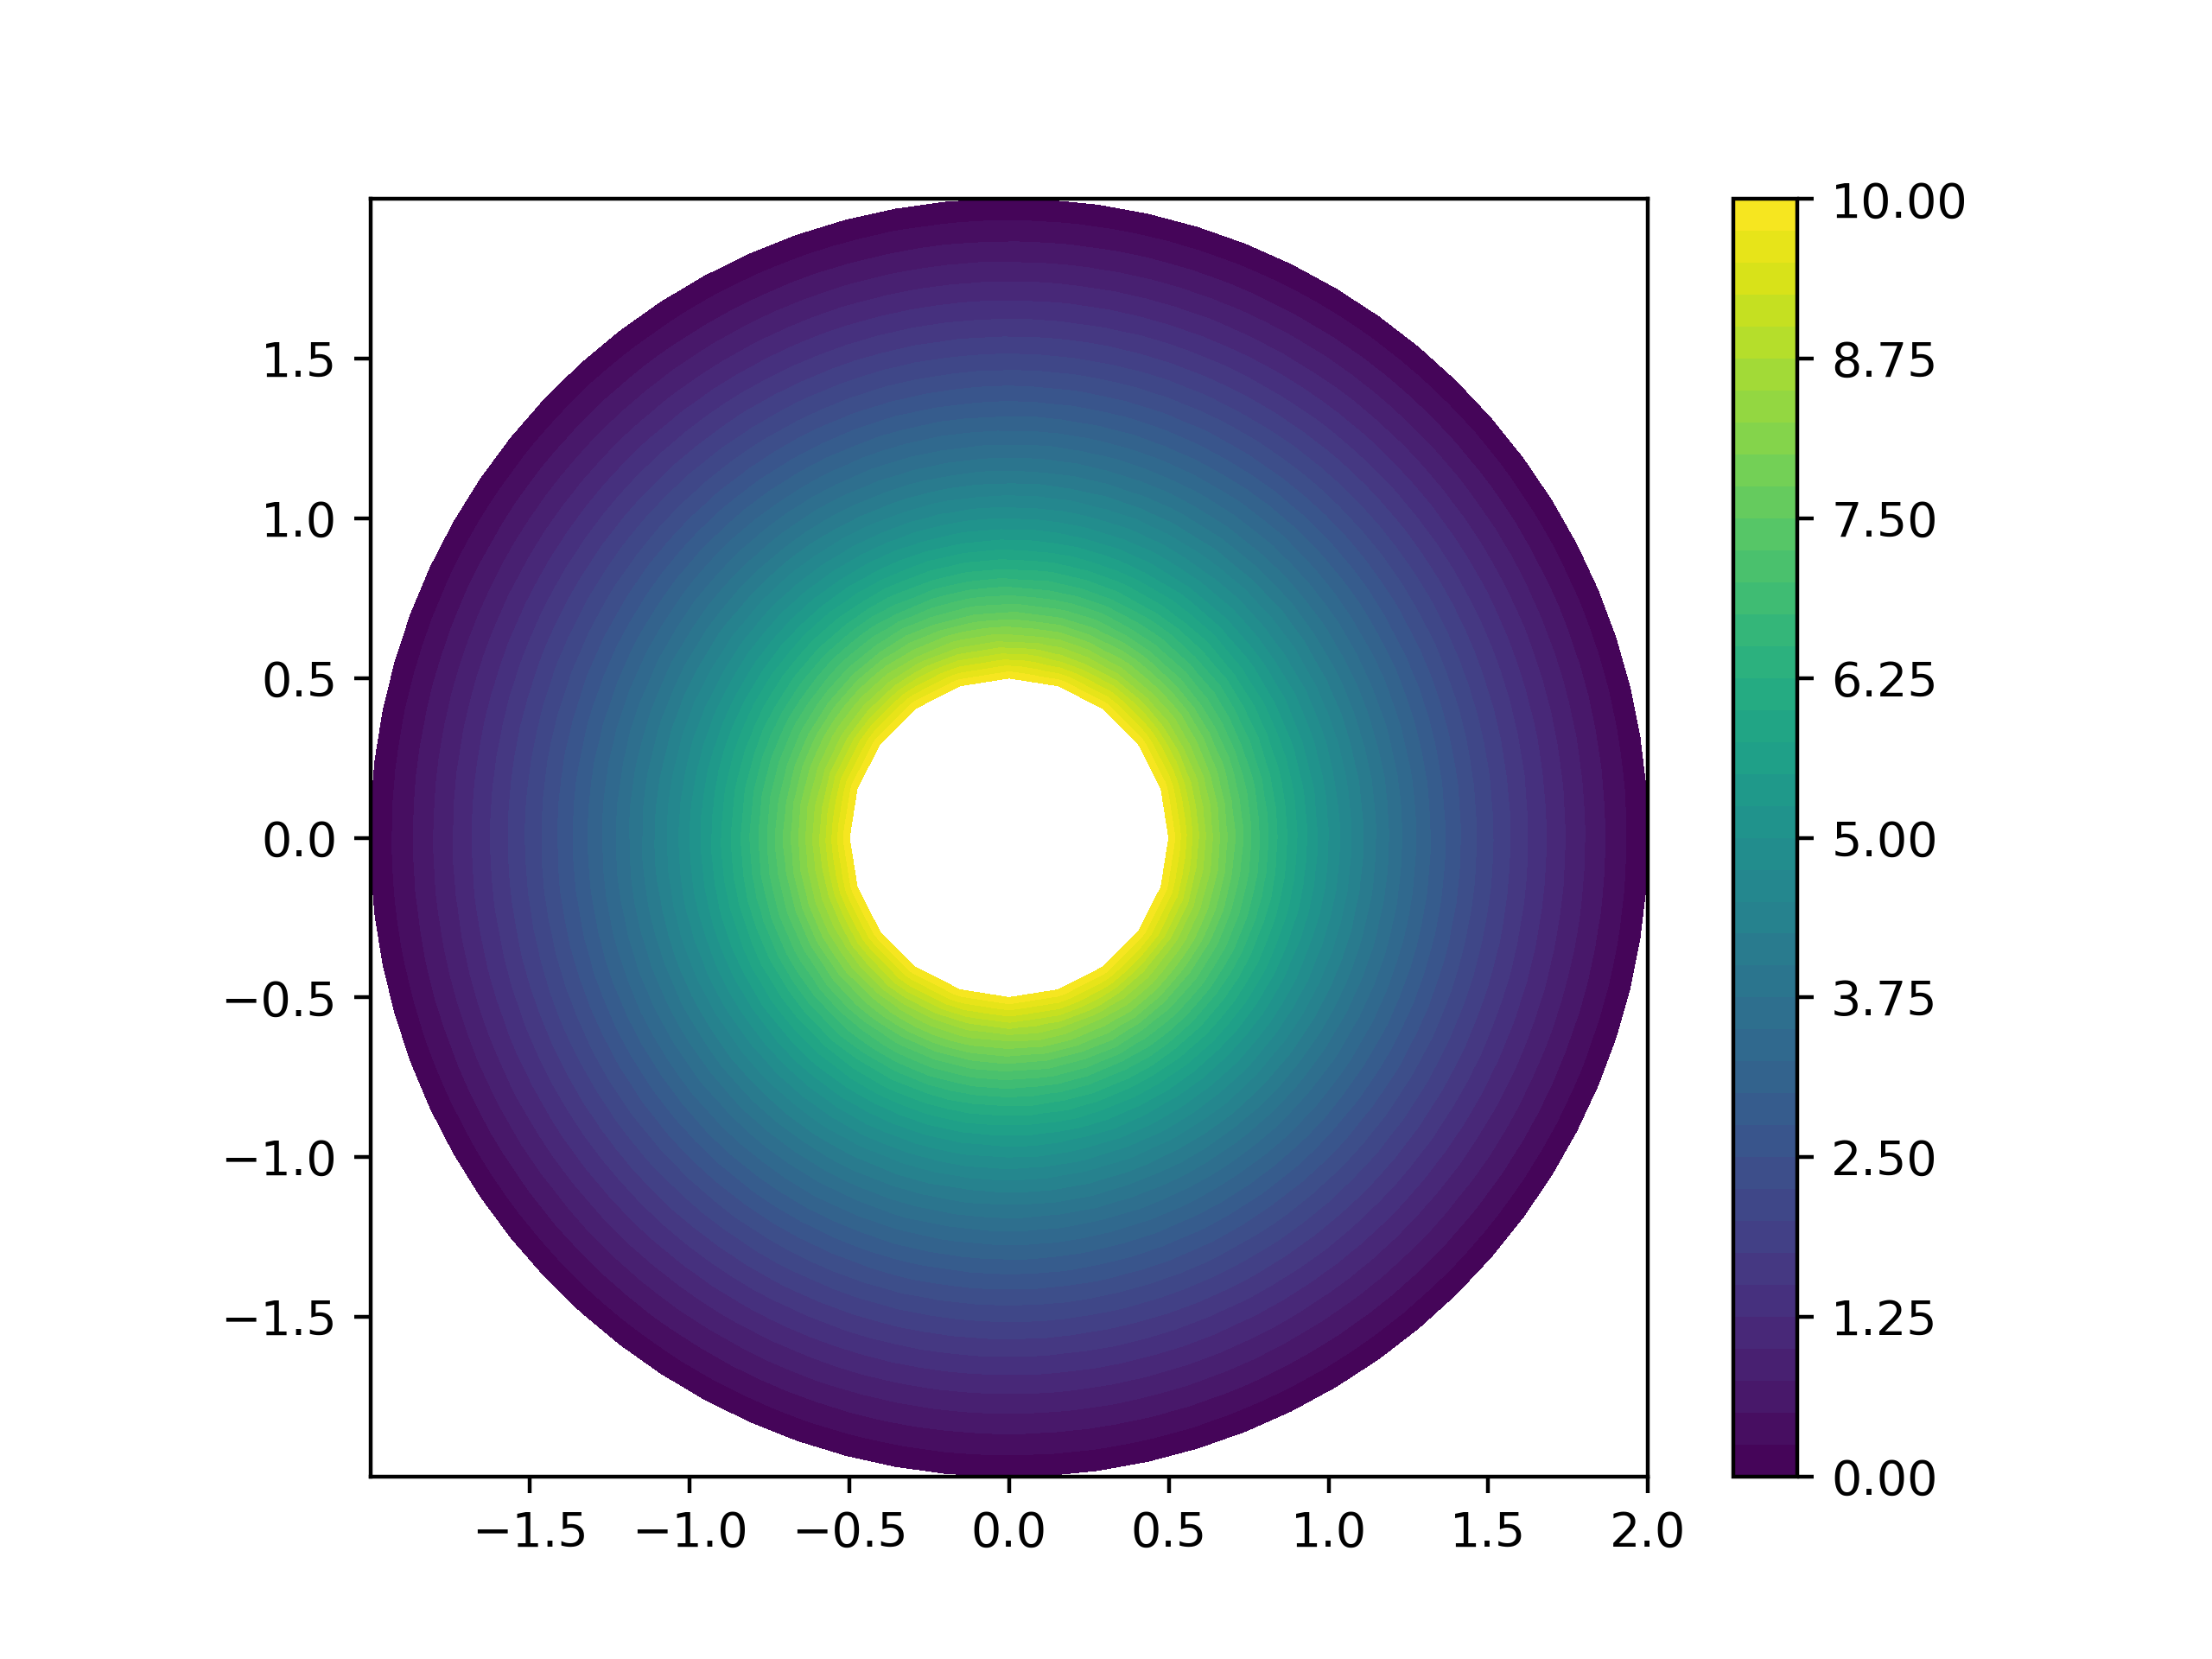
\includegraphics[width=\linewidth]{Figures/FEM/PotentialFieldFEMCoaxial.png}
    \caption{Coaxial Cable using Finite Element Method. In the left we have the solution for the potential while, on the right, we have the solution for the electric field.}
    \label{fig:VE_Fem}
\end{wrapfigure}
\begin{wrapfigure}{R}{0.4\linewidth}
    \centering
    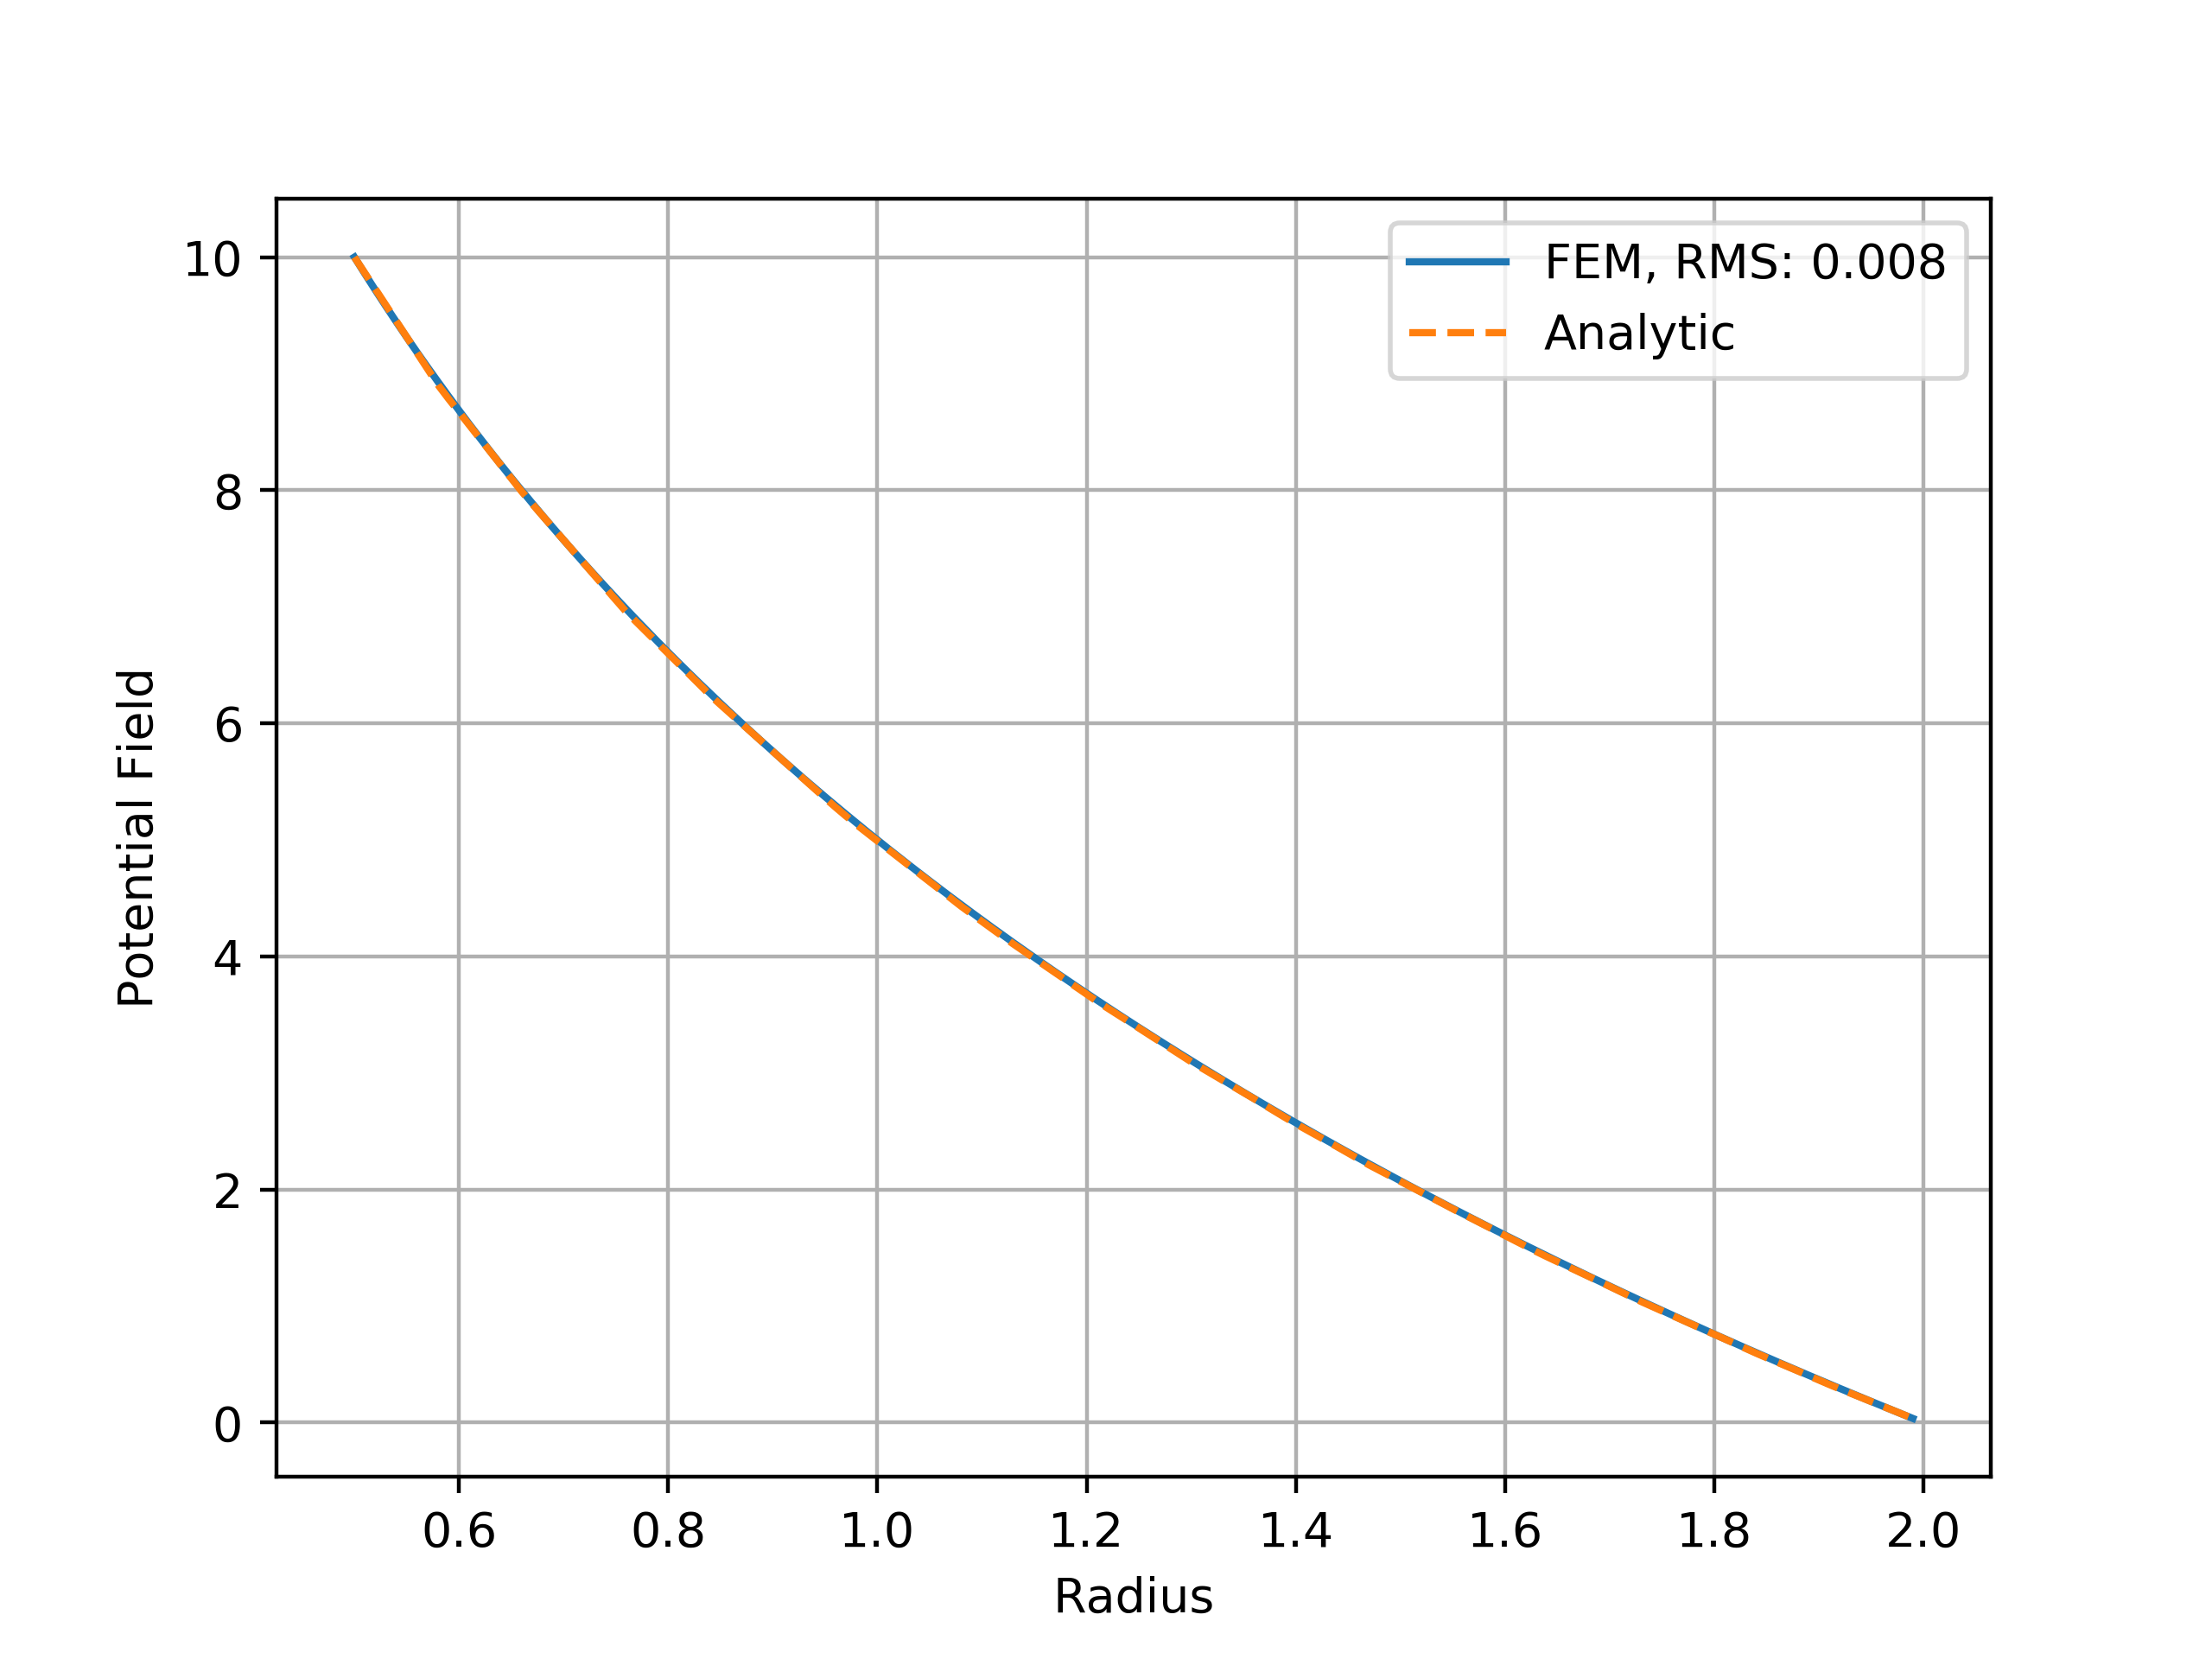
\includegraphics[width=\linewidth]{Figures/FEM/ComparissonPotentialFEMCoaxial.png}
    \caption{Coaxial Cable using Finite Element Method. In the left we have the solution for the potential while, on the right, we have the solution for the electric field.}
    \label{fig:VE_Fem}
\end{wrapfigure}
\end{comment}

\begin{wrapfigure}[13]{R}{0.38\linewidth}
    \centering
    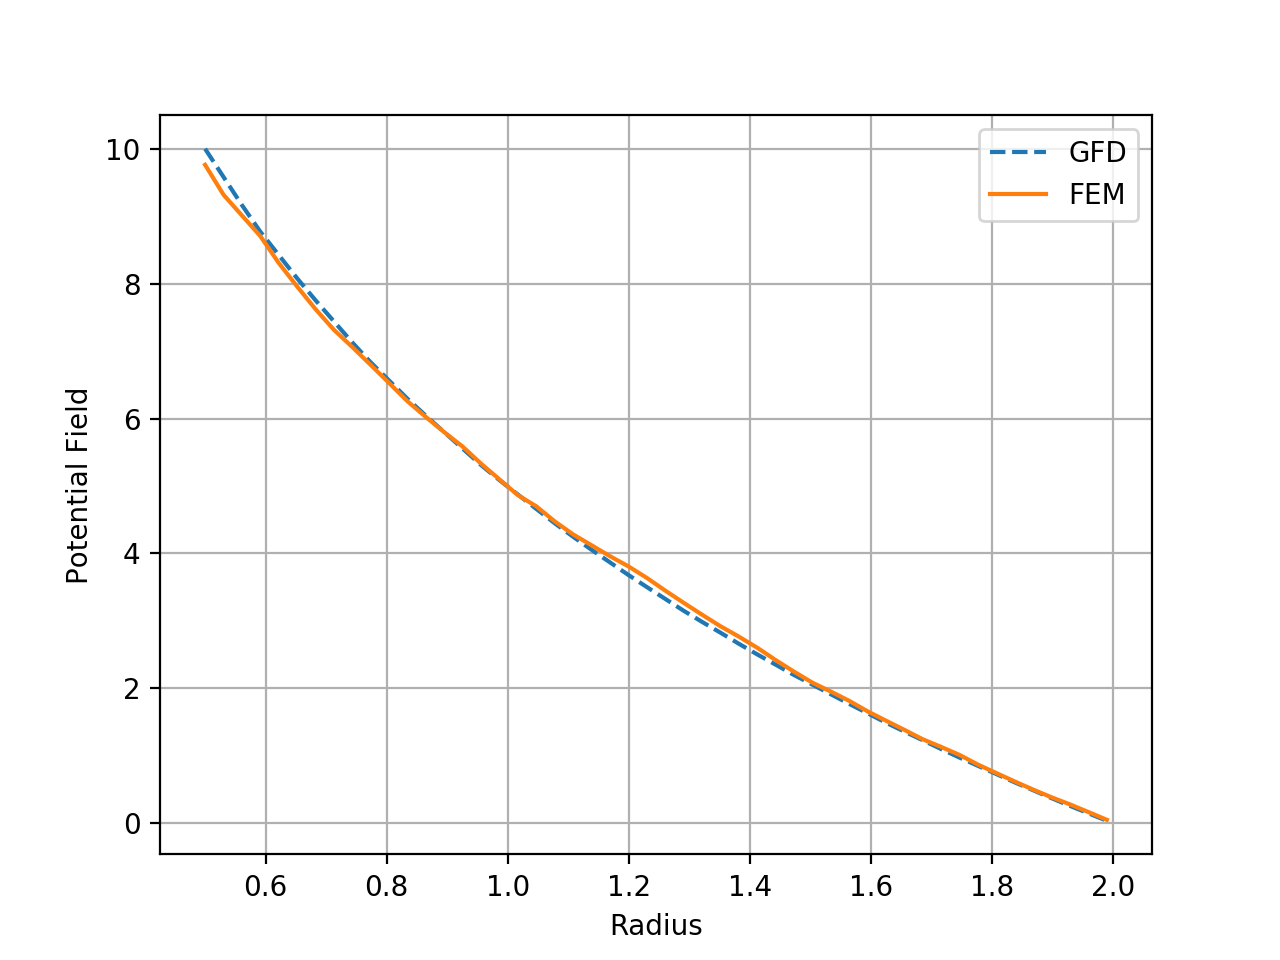
\includegraphics[width=0.9\linewidth]{Figures/FEM/ComparissonPotentialFEMGFD.png}
    \caption{Potential field plot as function of the radial distance.The orange line refers to the solution using the FEM approach whereas the blue line refers to the solution using GFD.}
    \label{fig:GFDvFEM}
\end{wrapfigure}

Upon comparing the obtained results with the analytical potential presented in Figure \ref{fig:gfdm_coax_solutions}, a noteworthy alignment is observed, showcasing a high degree of correspondence. In Figure \ref{fig:VE_Fem}, we juxtapose the analytical solution with the actual potential values, and we calculate the RMS for the solution. In the Appendix, electric field figures are included, and both scenarios exhibit a commendable conformity in terms of the solution. Notably, achieving the calculation of the electric field alongside the potential solution using FEM for a non-trivial geometry is a significant and promising outcome. We have opted to delve into more intricate geometries. However, given their heightened complexity, deriving an analytical solution proves challenging. Nonetheless, obtaining an approximate solution is feasible. These findings are elucidated in the Appendix. Subsequently, we extended our exploration to solve a problem termed the "coaxial dolphin." In both cases, the discernible influence of tips, a well-known phenomenon in the realm of electromagnetism, is evident.

% \begin{figure}
% \begin{center}
% 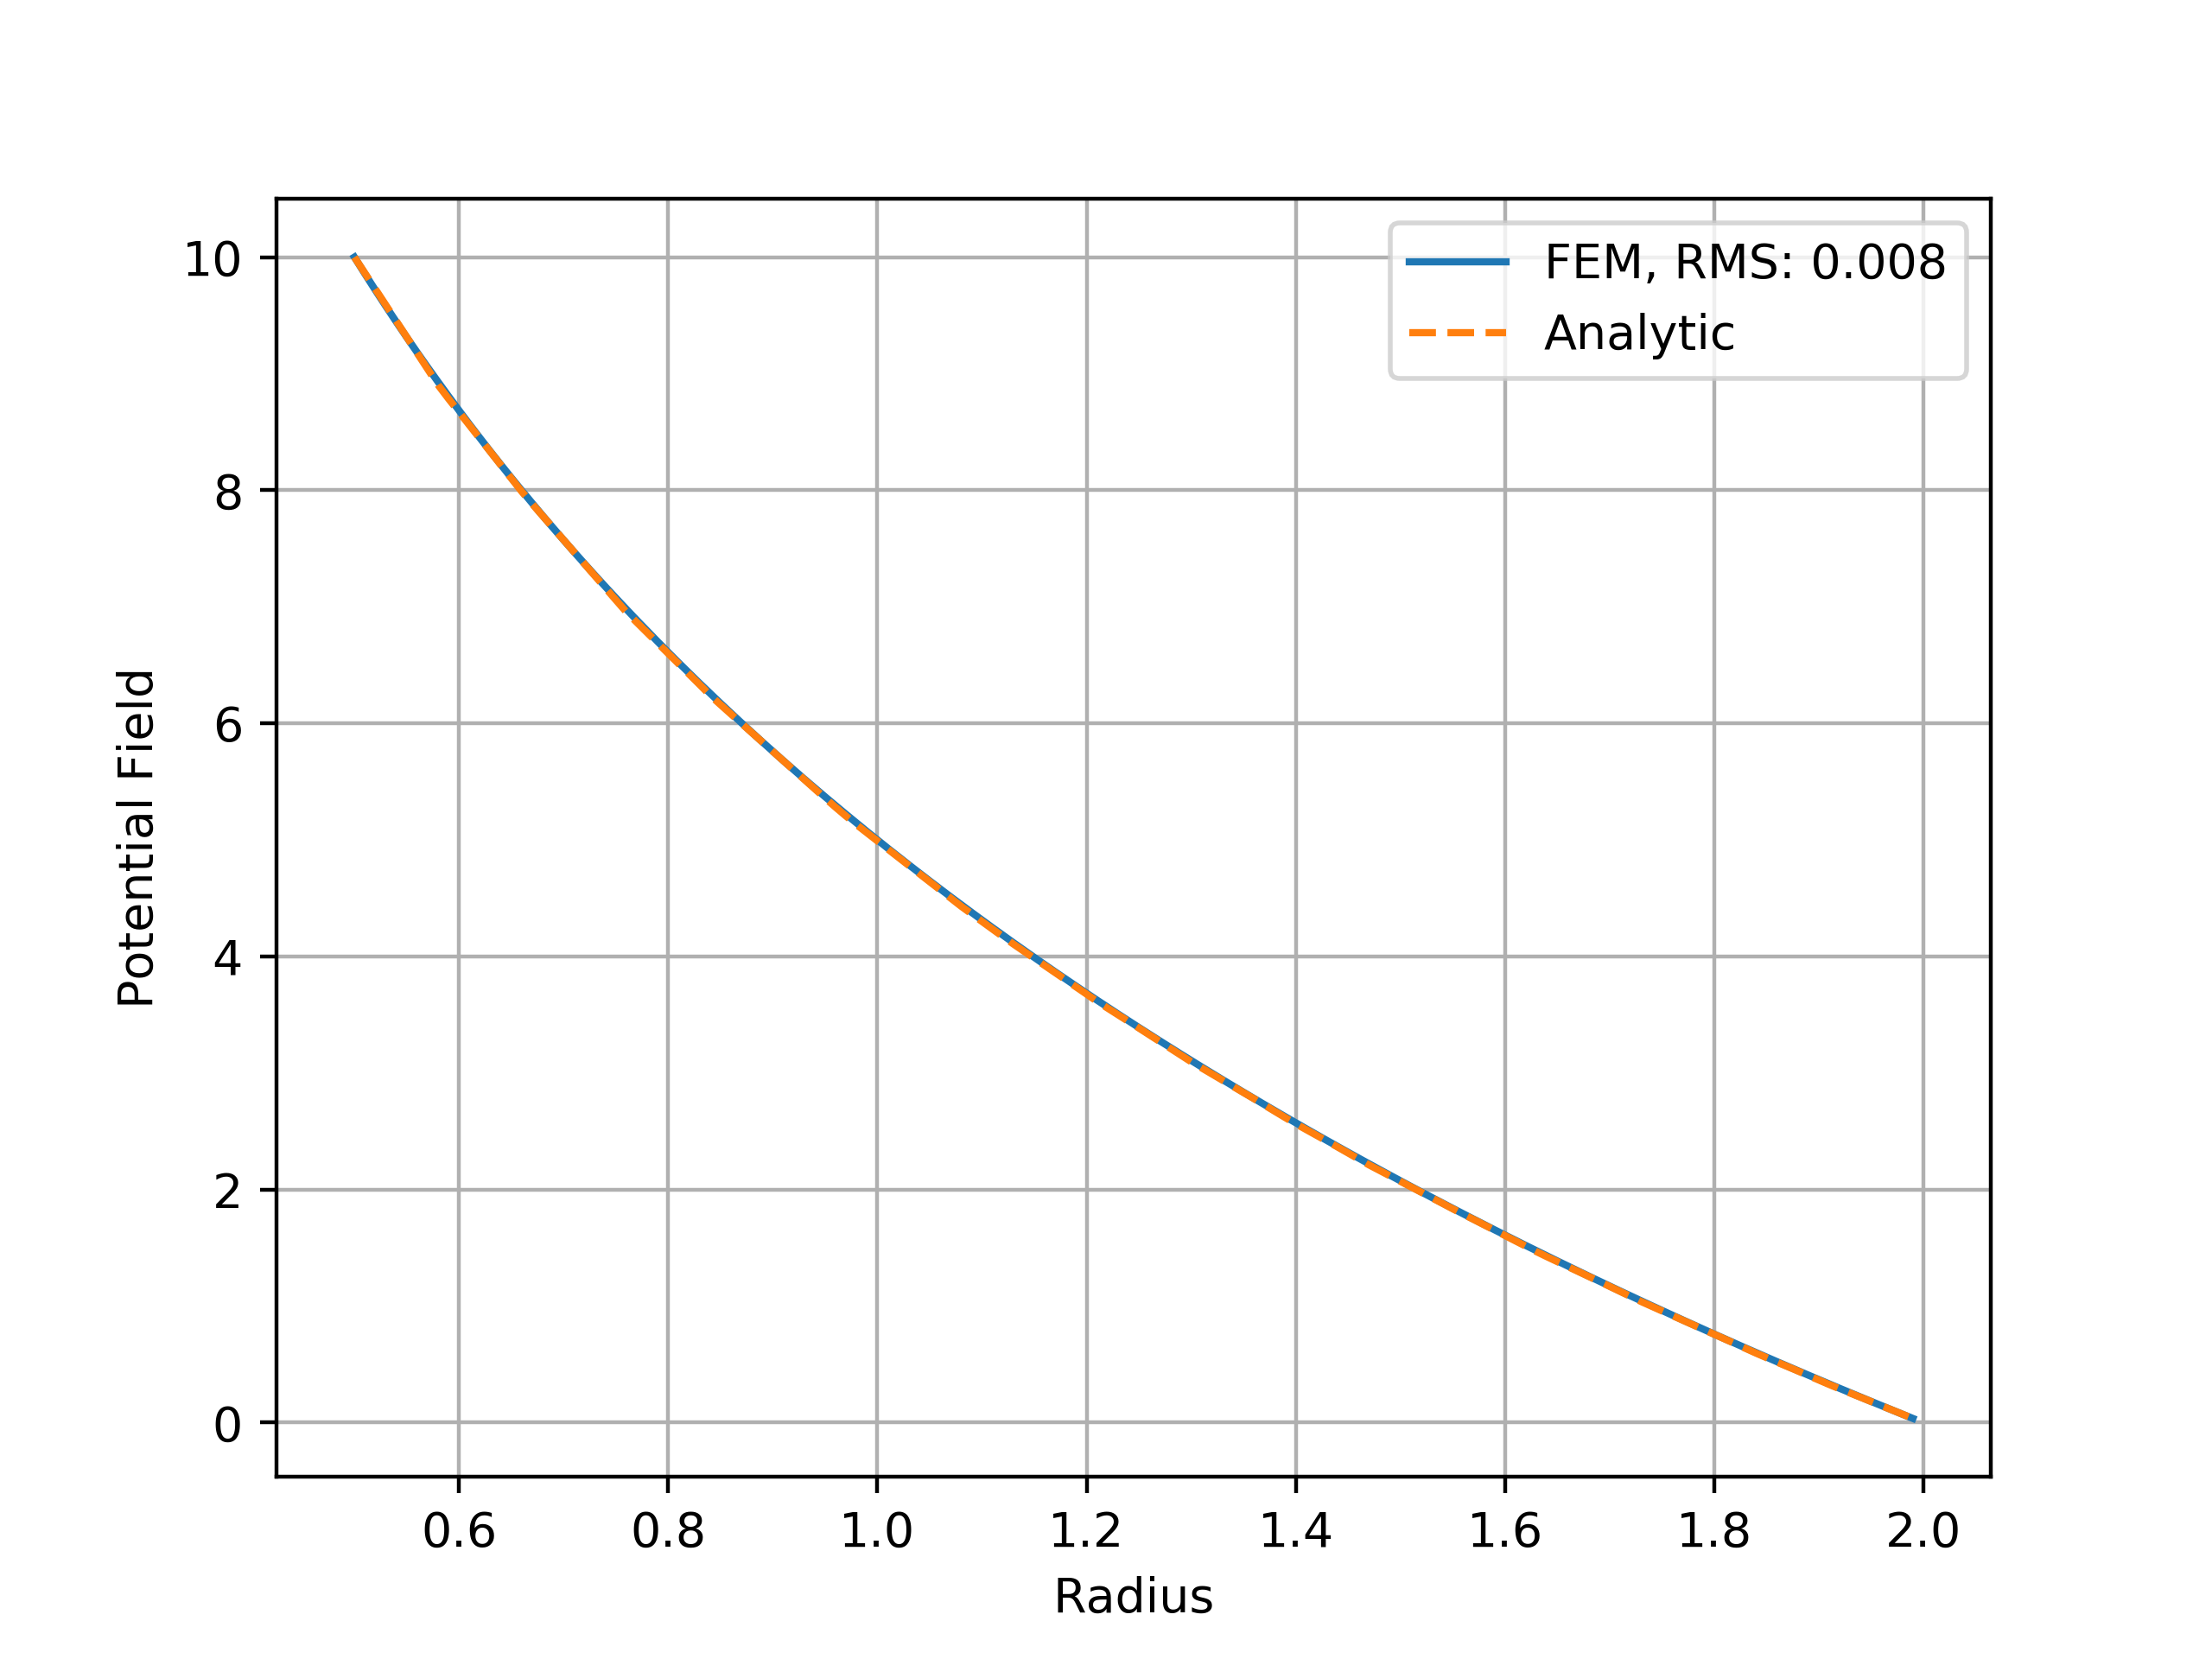
\includegraphics[width=0.75\textwidth]{Figures/FEM/ComparissonPotentialFEMCoaxial.png}
% \caption{Presentation of the potential (left) and electrical field (right) plots for both analytical and approximated solutions. The root mean square (RMS) for the potential is quantified at 0.008, whereas for the electric field, the RMS is measured at 0.167. This alignment is consistent with the schematic portrayal of the plots.}
% \label{fig:VE_Fem}
% \end{center}
% \end{figure}

% \begin{figure}
% \begin{center}
% 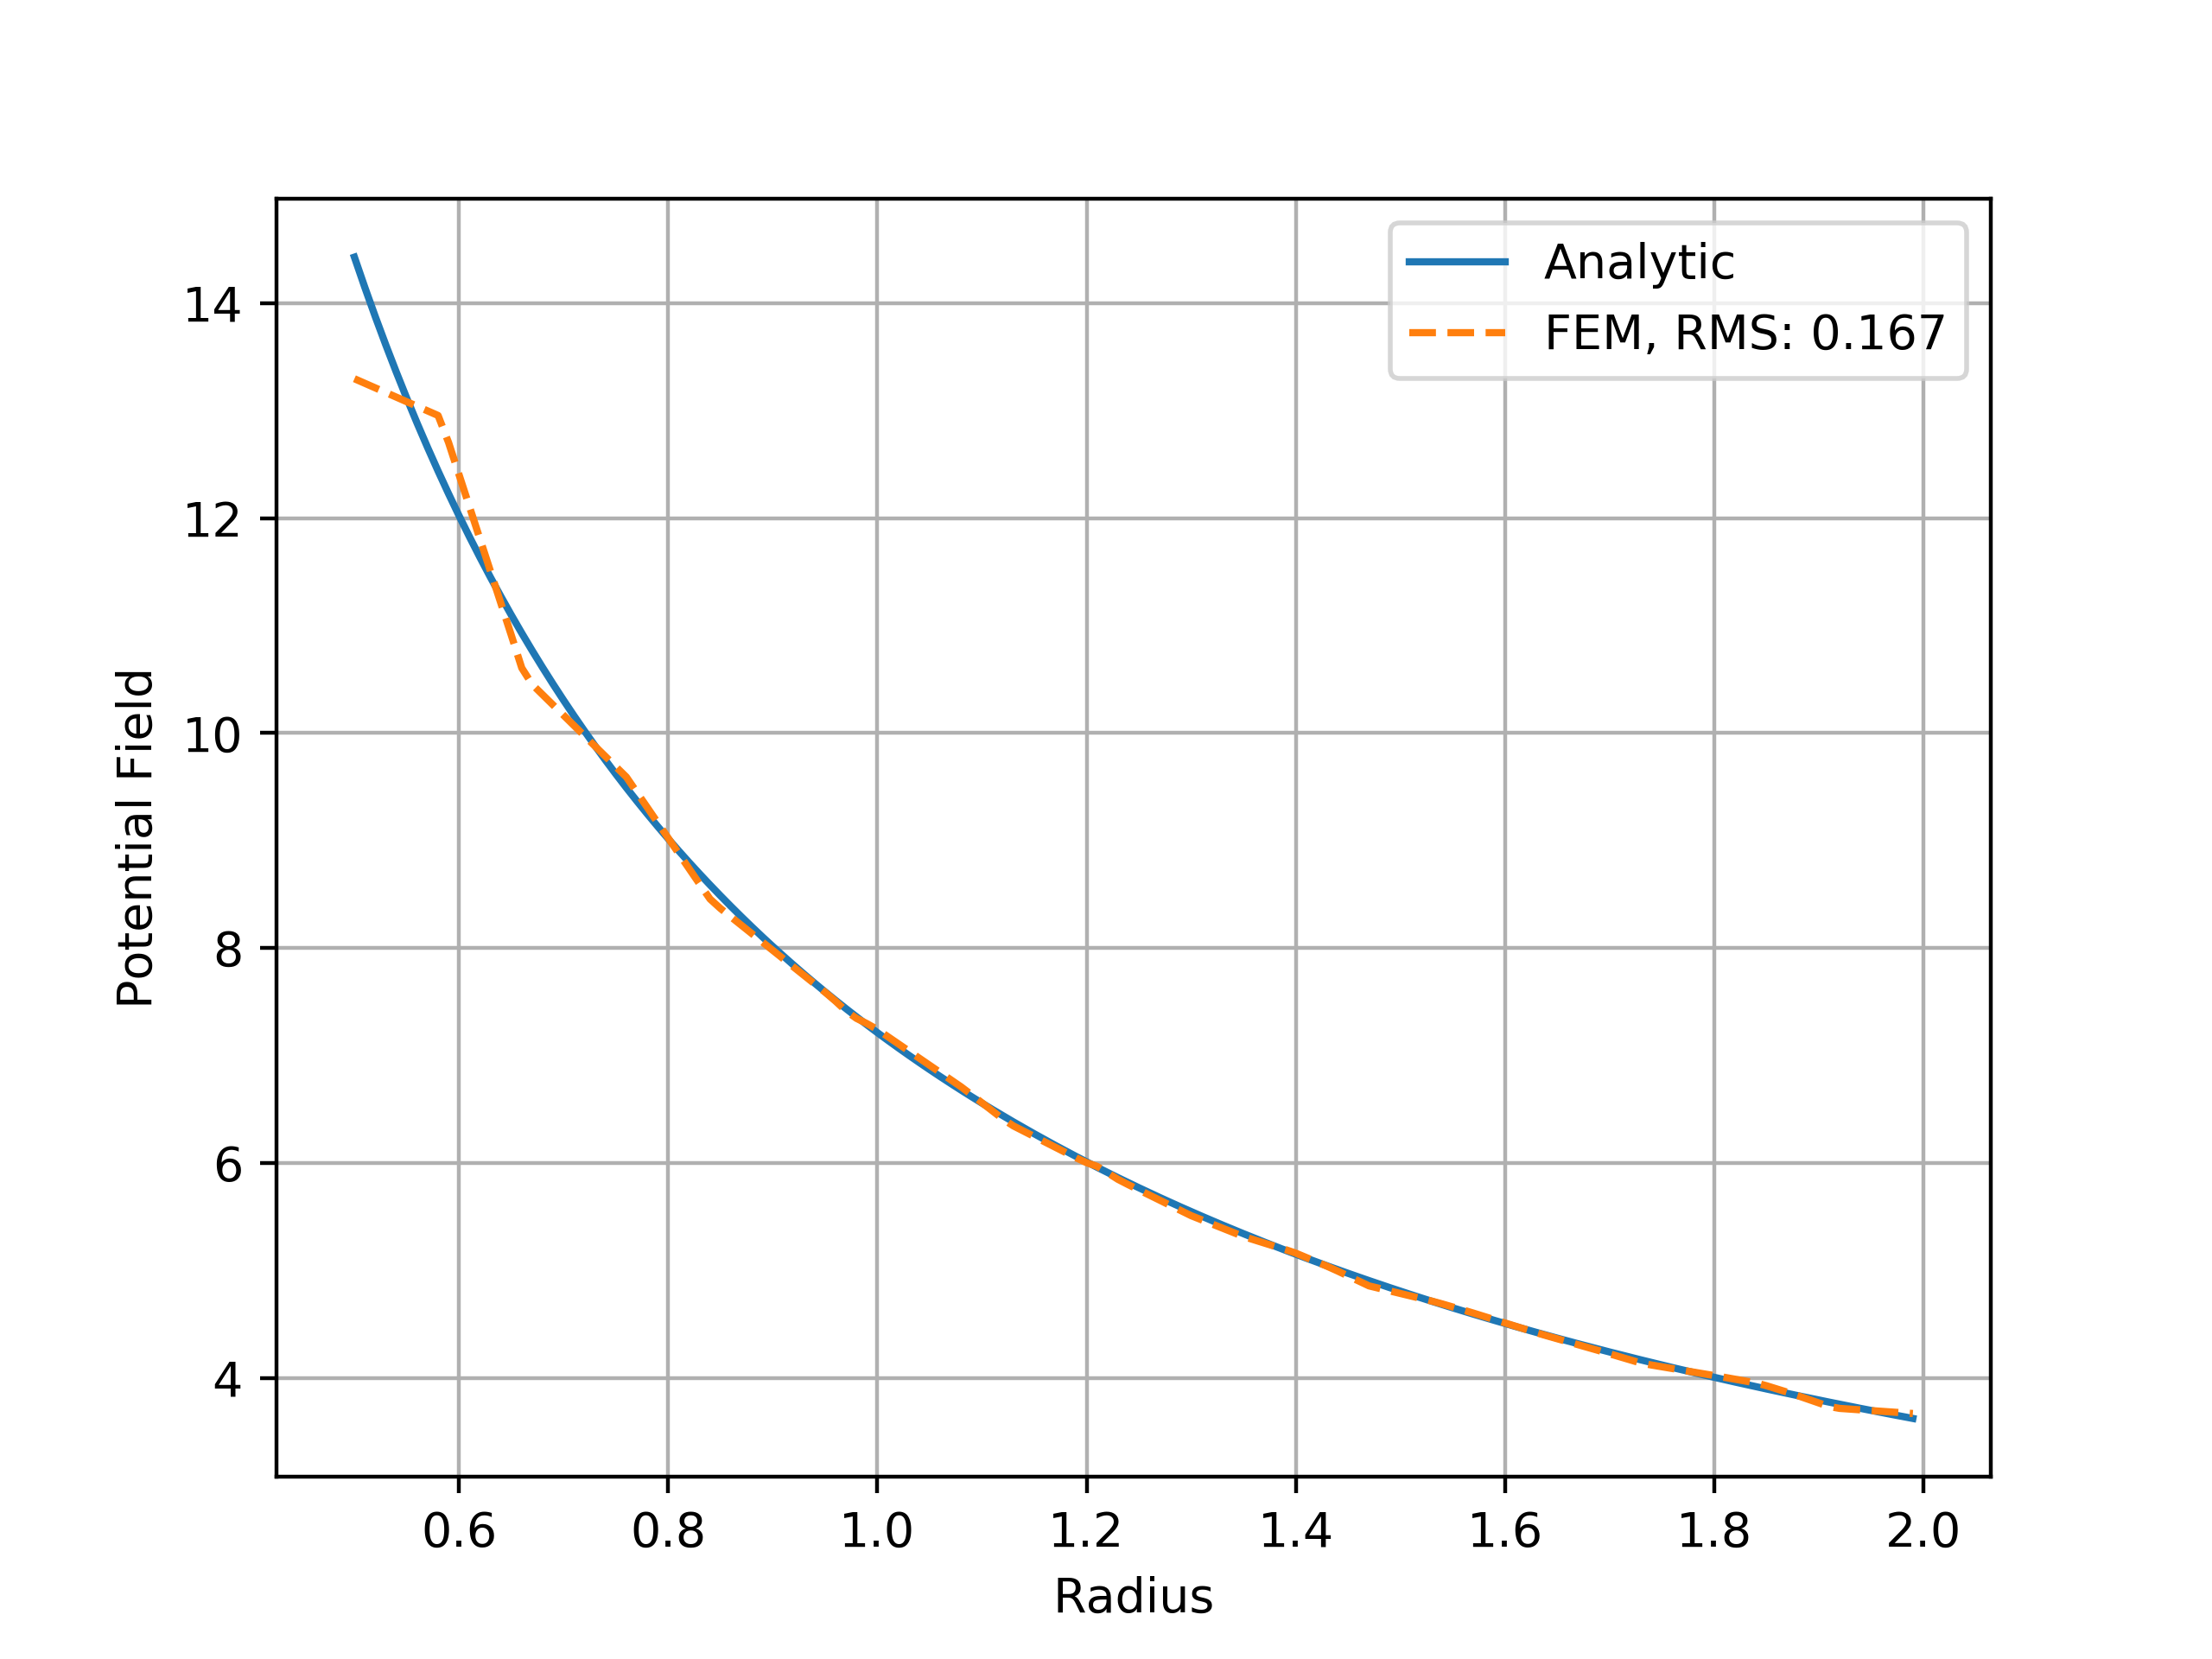
\includegraphics[width=.5\textwidth]{Figures/FEM/ComparissonEFieldFEMCoaxial.png}
% \caption{Coaxial Cable using Finite Element Method.}
% \label{fig:VE_Fem}
% \end{center}
% \end{figure}

\subsection{Comparison between both approaches}
\begin{comment}
\begin{figure}[hbt]
    \centering
    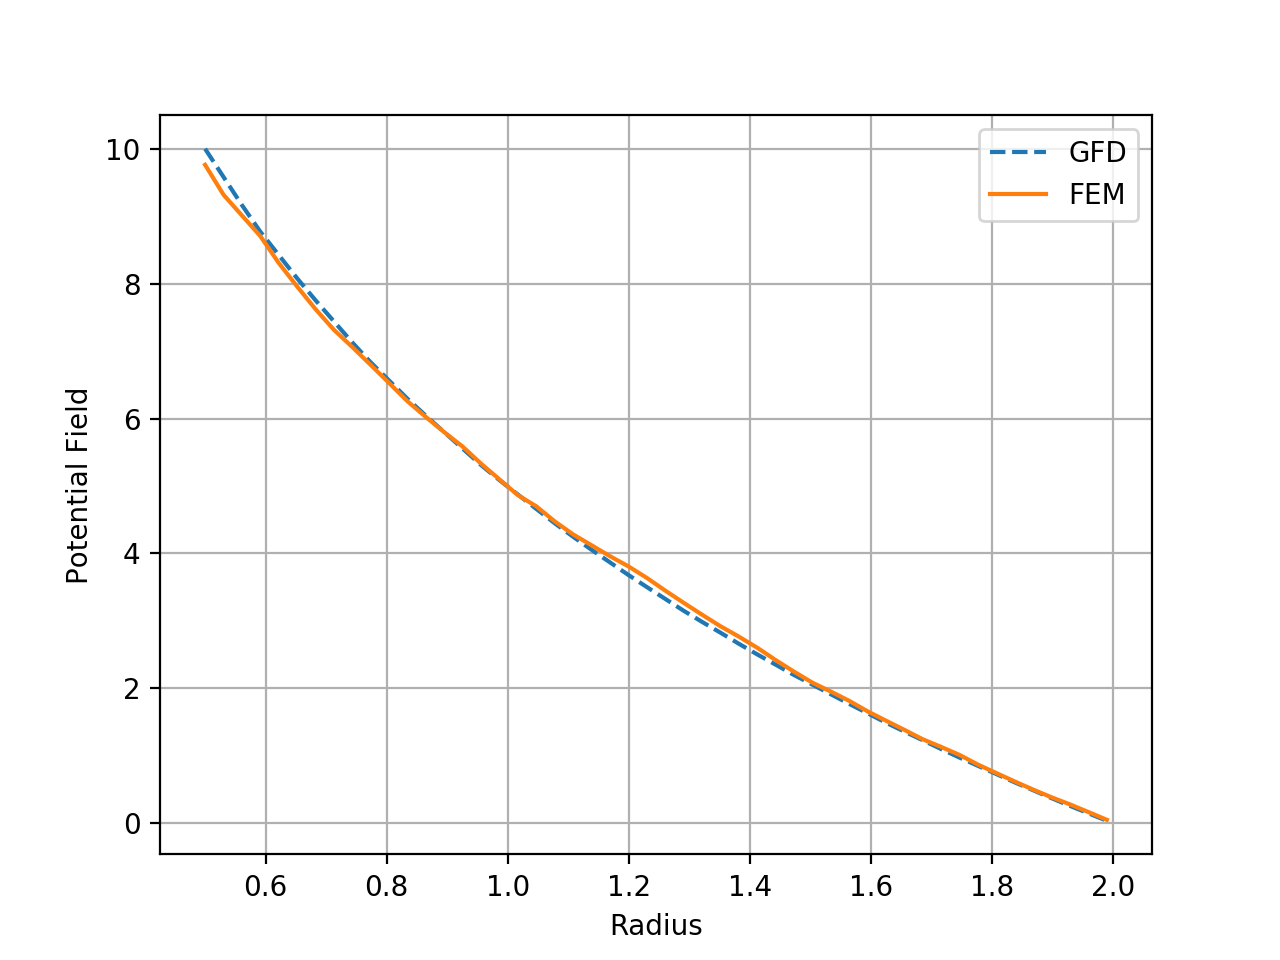
\includegraphics[width=\linewidth]{Figures/FEM/ComparissonPotentialFEMGFD.png}
    \caption{Comparison between the potential field with both approaches.}
    \label{fig:GFDvFEM}
\end{figure}
\end{comment}

Finally, we decided to compare both methods and examine the relationship between them. In Figure \ref{fig:GFDvFEM}, we present the potential graph obtained using both approaches, given the symmetry of the system we just fix some arbitrary radius and sample the potential. It is evident that we achieve a commendable performance in both solutions, aligning well with the original solution, as discussed earlier. Importantly, it should be highlighted that with the proposed methodology, we were able to approximate the precision of the Finite Element Method (FEM) to a certain extent. This achievement is noteworthy as it allows us to explore more intricate geometries without the need for employing FEM, which is considerably more complex.

\section{Conclusion}
We have presented a new method for solving Laplace's equation, the GFDM. The method performs with slightly worse error compared to the FEM but is notably easier to implement. The GFDM has been designed for generality and ease of use even for irregular geometries. The method is intuitive, easy to understand, and leaves intermediate steps accessible to the user. The FEM method is unintuitive, difficult to tune with confidence, and resembles a "black box" approach to the problem. Although the FEM has converged to a solution for the coaxial problem with higher accuracy, the GFDM has achieved similar accuracy with a more intuitive approach.

In the near future, we intend to test the GFDM on irregular geometries to test agreement with the FEM. Various improvements to the GFDM can be done, including more intuitive suggestion of appropriate hyper-parameters, allowance of holes in boundaries, and periodic boundary conditions. We would like to improve the neighbor selection step by using a graph-traversal approach. We also acknowledge that we claim the GFDM converges to a solution more quickly than the Cartesian FDM for irregular geometries without demonstration. Implementing a Cartesian FDM to test for a slower convergence for some irregular geometry is warranted.

\FloatBarrier
\newpage

\bibliography{Bibliography}
\bibliographystyle{acm}

\appendix

\section{Extras}

This appendix presents the results of FEM and GFD, including:

\begin{itemize}
    \item Mesh visualization 
        \begin{itemize}
            \item We display the mesh used for the FEM solution using for the coaxial cable, highlighting the chosen spatial discretization.
            \item We also present the mesh used for the two conducting bars and the conducting dolphin.
        \end{itemize}
    \item Complex geometries: to demonstrate the versatility of the new approach, we analyze two additional scenarios with more complex geometries:
    \begin{itemize}
        \item Two conducting bars: We compare the potential distributions for two conducting bars in close proximity using both approaches.
        \item Coaxial dolphin: We investigate the potential behavior in a dolphin configuration, consisting of a dolphin-shape conducting nested in a grounded square.
    \end{itemize}
        

    \item Error Analysis:
        \begin{itemize}
            \item We assess the accuracy between solutions by calculating the absolute error for both the two conducting bars and the coaxial geometry.
            \item It's important to note that the exact same mesh was used for both scenarios, allowing for a direct comparison of the error behavior.
        \end{itemize}
\end{itemize}


\begin{figure}
\begin{center}
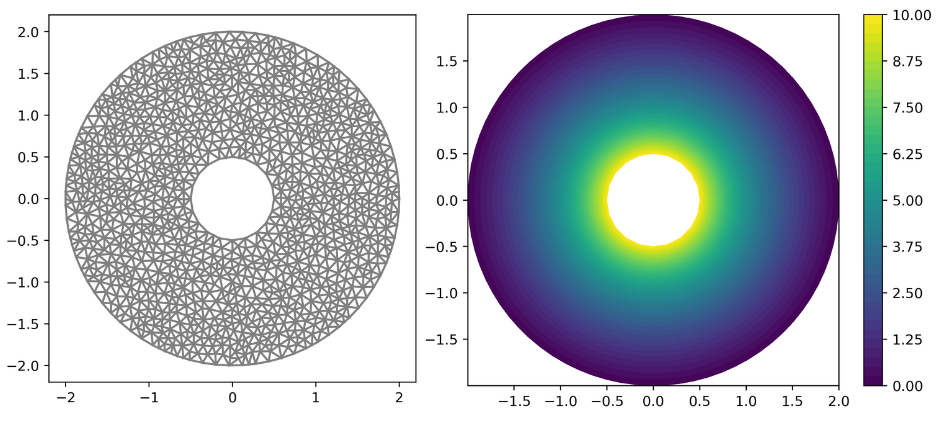
\includegraphics[width=.85\textwidth]{Figures/FEM/CoaxialMeshandV_FEM.png}
\caption{Right: Mesh of the domain $\Omega$ in which we solve the Laplace equation using the FEM approach. As we can observe, the partition of the domain is not regular, and in fact this is what allow us to explore a wider range of complex geometries.Left: solution for the potential field, as mentioned in the section about FEM, it's important to notice that we have the information on every point of the domain that's why we're able to have a plot with such accuracy.}
\label{fig:FEM_Mesh_and_Potential}
\end{center}
\end{figure}

\begin{figure}
\begin{center}
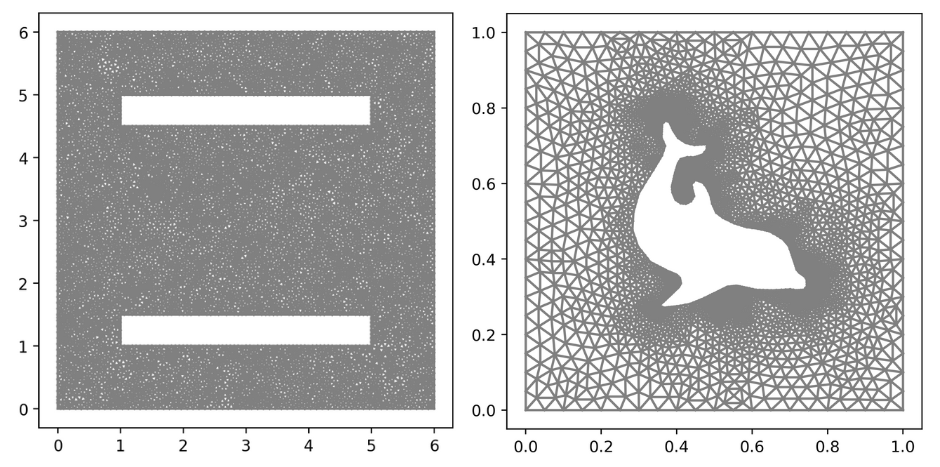
\includegraphics[width=.95\textwidth]{Figures/FEM/Meshes.png}
\caption{Right: Mesh used for the two conducting bars problem, note that the mesh is highly dense. Left: Mesh used for the coaxial dolphin, note how the mesh is more dense in some zones, that;s because we need a better precision in those domains.}
\label{fig:Meshes}
\end{center}
\end{figure}

% \begin{figure}
% \begin{center}
% 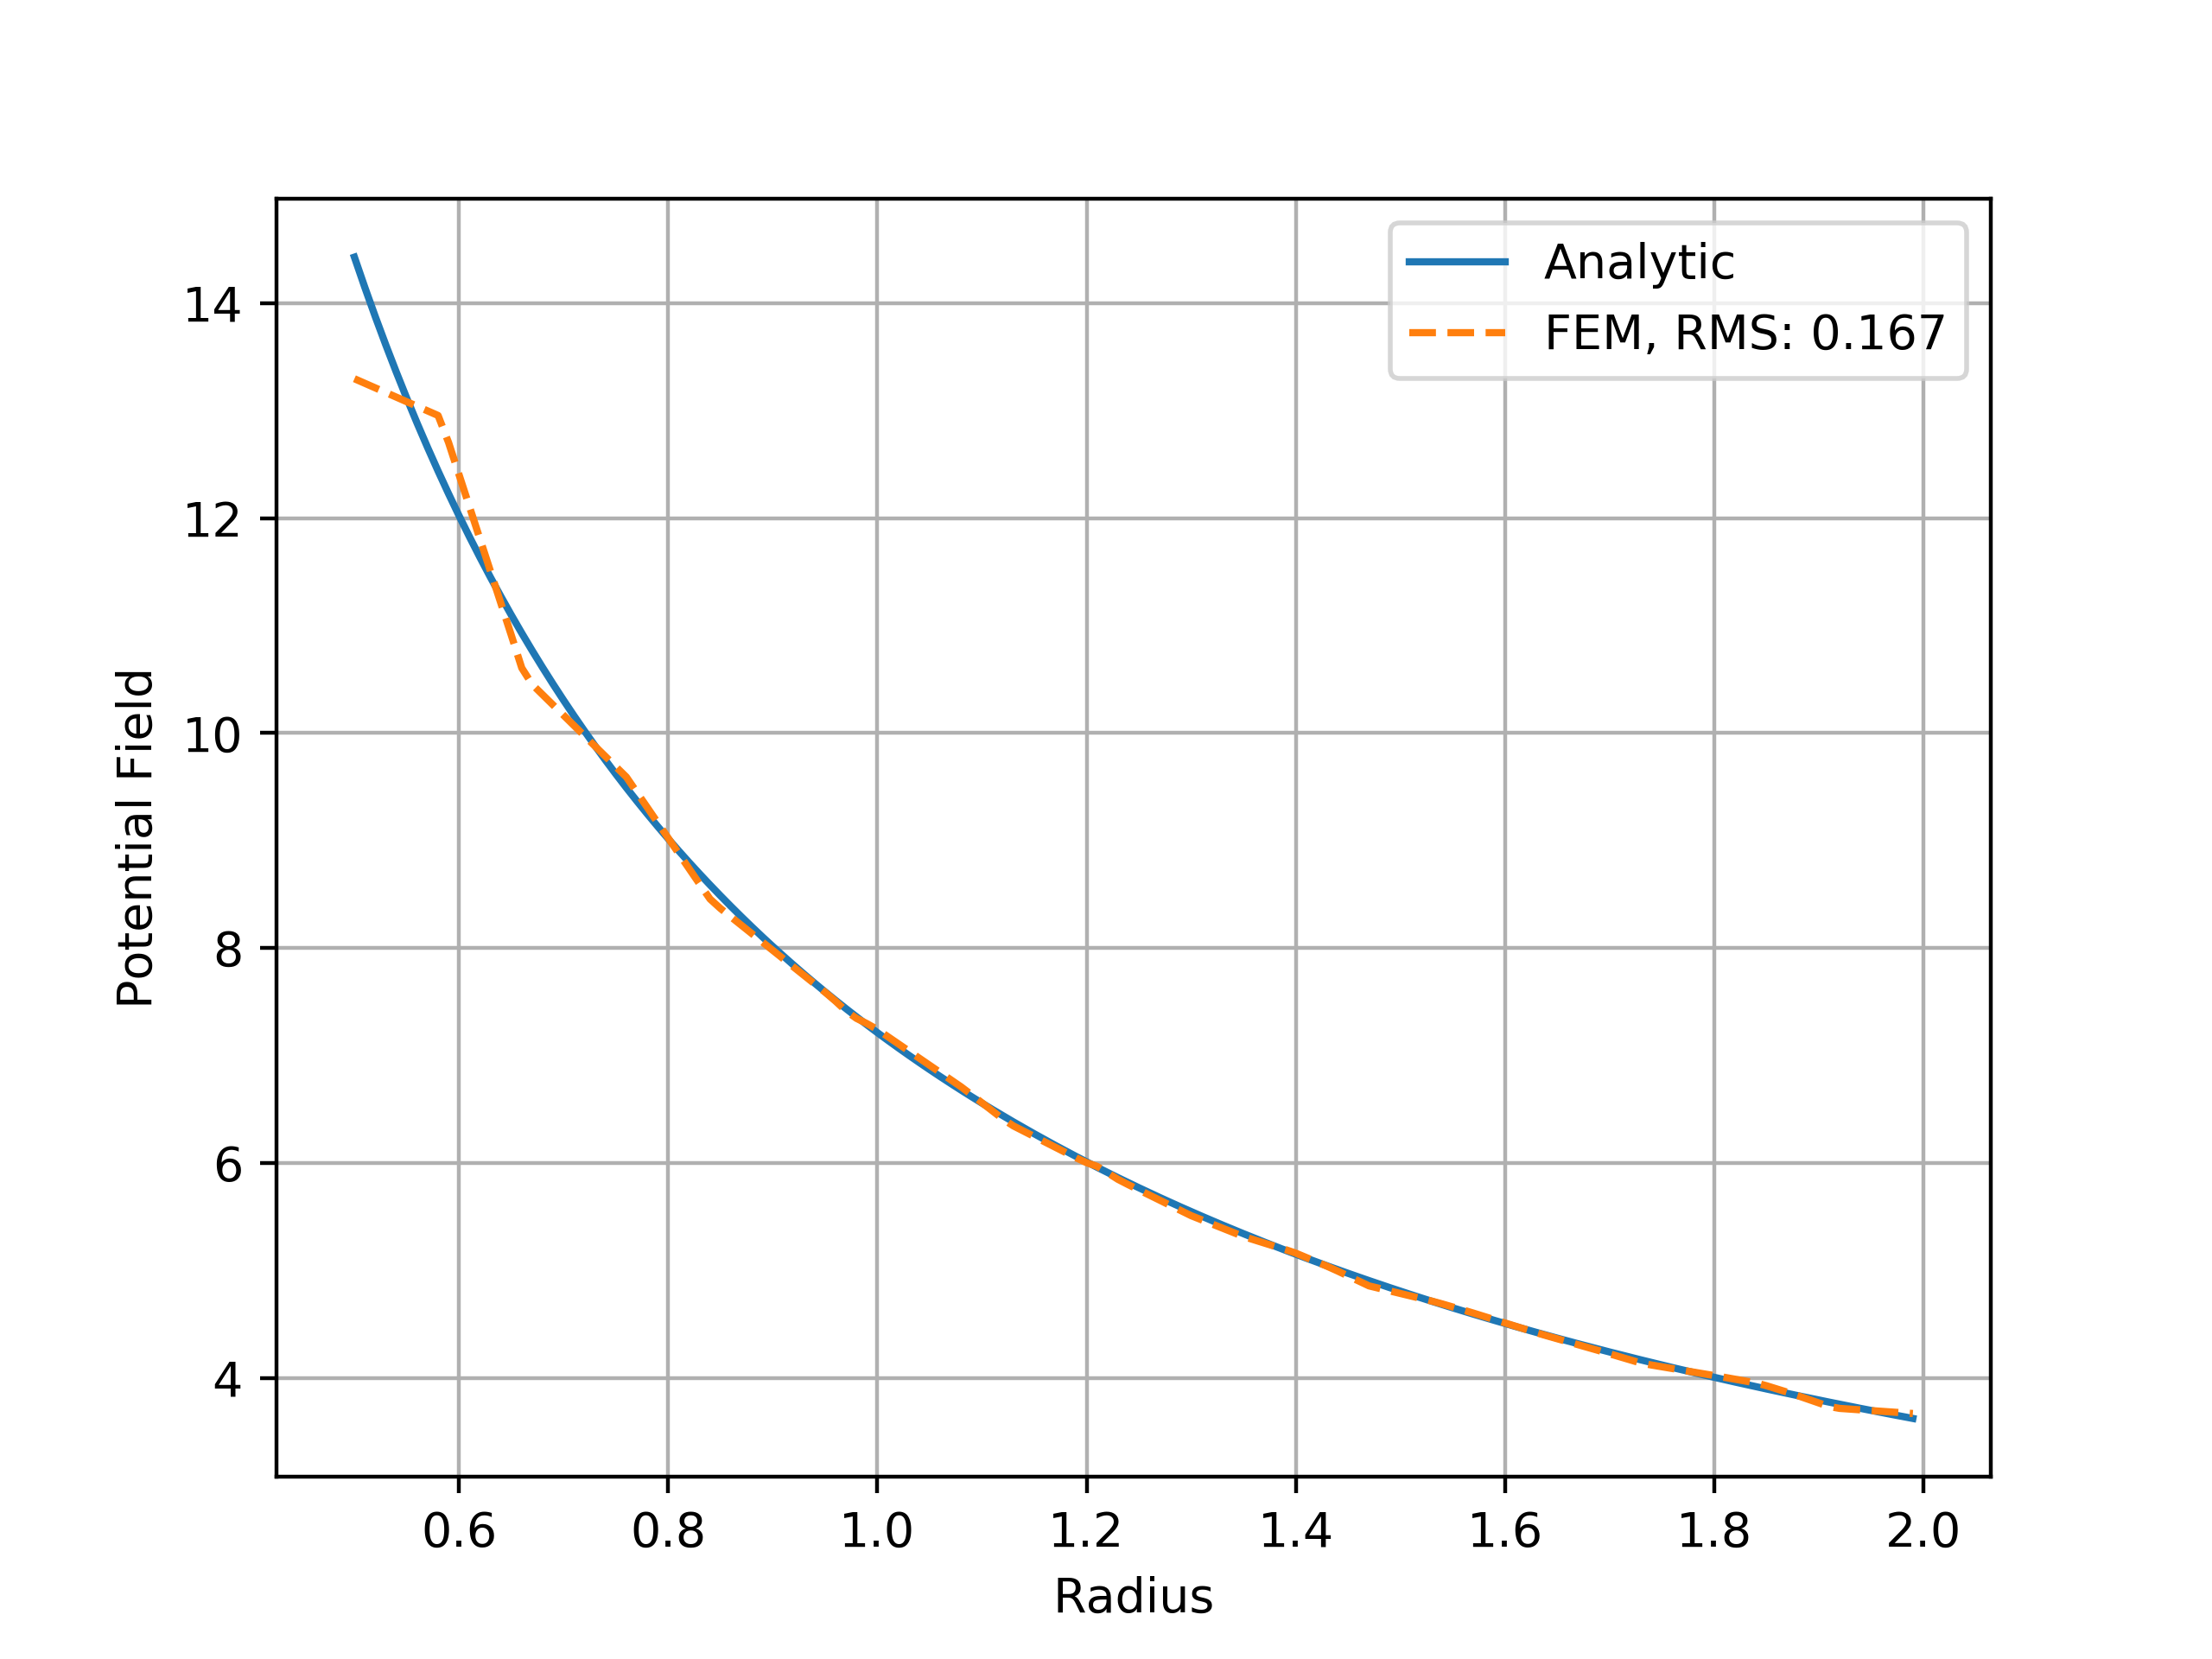
\includegraphics[width=.5\textwidth]{Figures/FEM/ComparissonEFieldFEMCoaxial.png}
% \caption{Coaxial Cable using Finite Element Method.}
% \label{fig:VE_Fem_Full}
% \end{center}
% \end{figure}

% \begin{wrapfigure}{R}{0.45\linewidth}
%     \centering
%     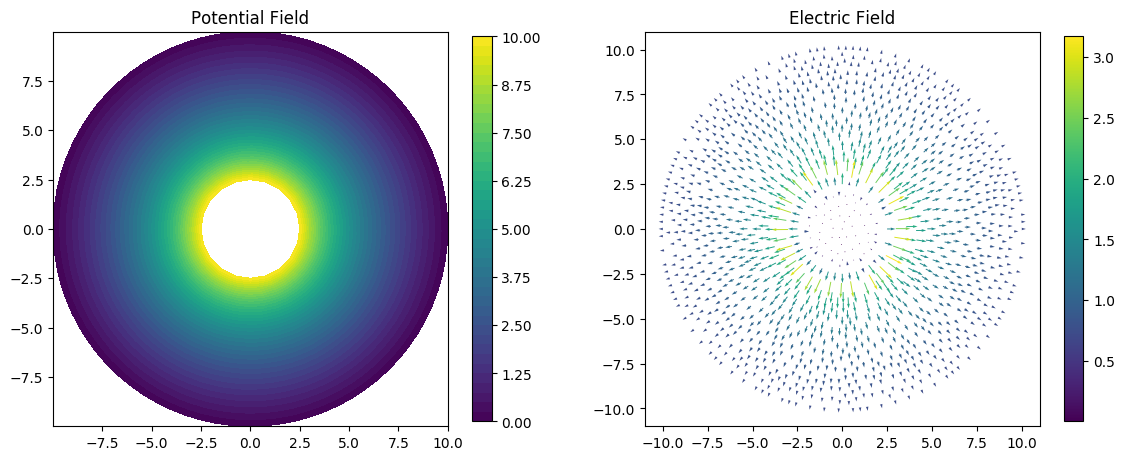
\includegraphics[width=\linewidth]{Figures/FEM/VE_Coaxial.png}
%     \caption{Coaxial Cable using Finite Element Method. In the left we have the solution for the potential while, on the right, we have the solution for the electric field.}
%     \label{fig:VE_Fem}
% \end{wrapfigure}

% \begin{figure}
% \begin{center}
% 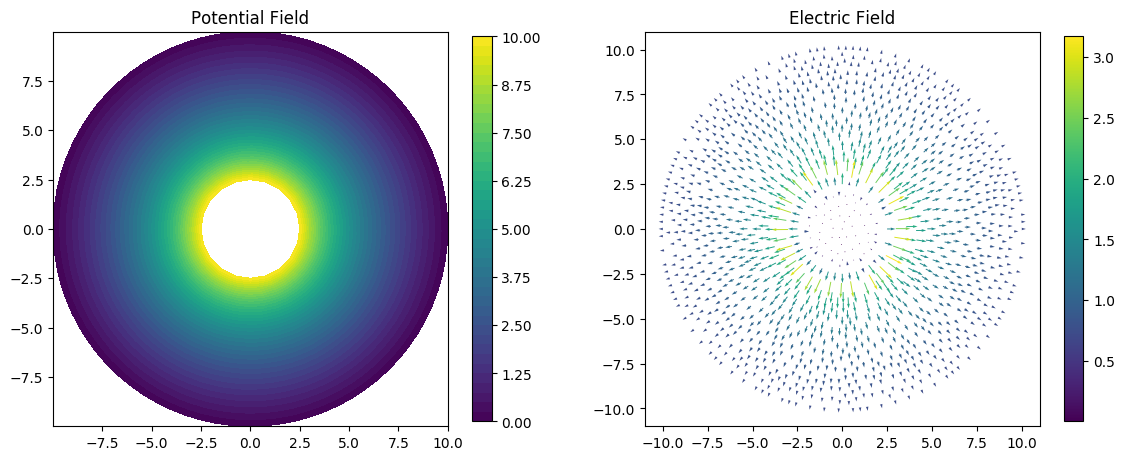
\includegraphics[width=.95\textwidth]{Figures/FEM/VE_Coaxial.png}
% \caption{Coaxial Cable using Finite Element Method. Left: solution for the potential field, as mentioned in the section about FEM, it's important to notice that we have the information on every point of the domain that's why we're able to have a plot with such accuracy. Right: with the information of the potential field we were able to plot the electric field, and again, we have the information on every point, but as usual with vector fields, we choose to plot just a few, in order to understand the behaviour of the field.}
% \label{fig:VE_FEM_FULL}
% \end{center}
% \end{figure}


% \begin{figure}
% \begin{center}
% 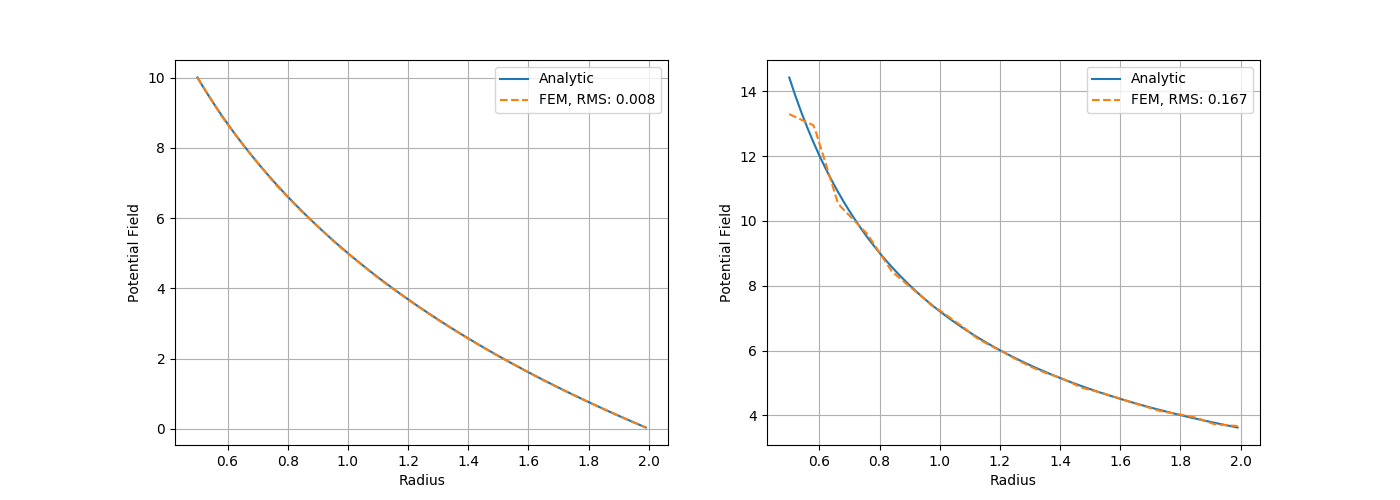
\includegraphics[width=.99\textwidth]{Figures/FEM/FullComparissonVECoaxial.png}
% \caption{Comparison between analytical and approximate solution for the Coaxial Cable. Left: we have the comparison between the potential field, and we can see that there's a very good fit between the solutions. Right: comparison between electric field, we have a slightly difference with the electric potential, but overall, the match is really close.}
% \label{fig:VE_FEM_FULL}
% \end{center}
% \end{figure}



\begin{figure}
\begin{center}
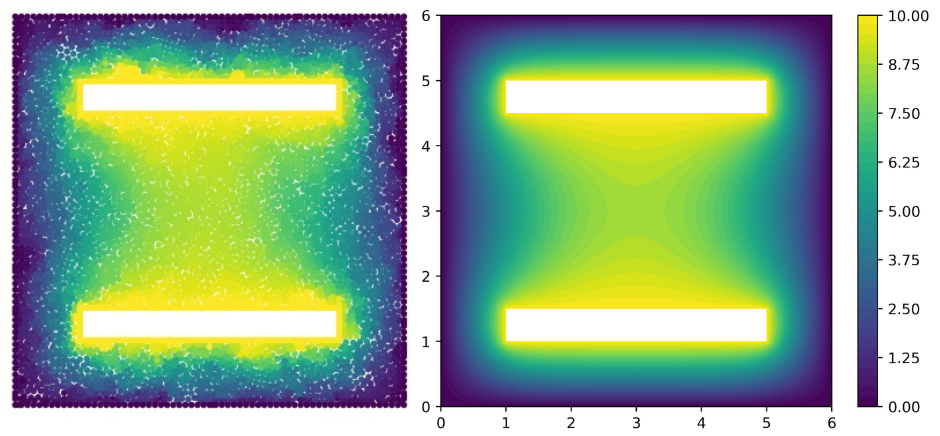
\includegraphics[width=.95\textwidth]{Figures/FEM/TwoBars_GFD&FEM.png}
\caption{Two conducting bars inside inside a square grounded. Left: Potential Field of two conducting bars inside a grounded square. Right: plot of the Electric Field, in which we can observe the how the electric field has a really strong value on the edges of the rectangles, which corresponds to a very well known phenomena in electromagnetic theory.}
\label{fig:VE_Dolphin}
\end{center}
\end{figure}

\begin{figure}
\begin{center}
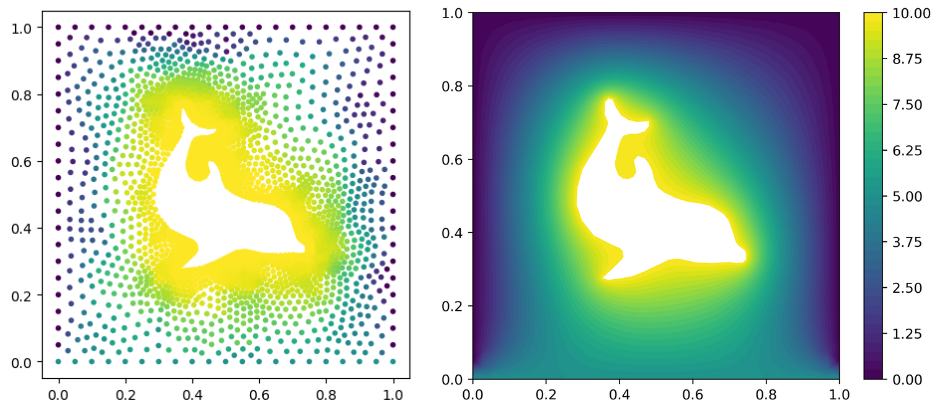
\includegraphics[width=.95\textwidth]{Figures/FEM/Dolfin_GFD&FEM.png}
\caption{Coaxial Dolphin solution for the potential field using both GFD and FEM approaches. Parameter of the problem: the dolphin is fix in potential at a value of 10 V, where the left, right and bottom sides are grounded, finally, the bottom is set to a value of 5 V. Left: solution using GFD approach. Right: solution using FEM approach. For this problem we decided to use the solution given by FEM as an analytical solution and compare with GFD: as we can see qualitatively the solutions are quite similar.}
\label{fig:VE_Dolphin}
\end{center}
\end{figure}
\begin{figure}
    \centering
    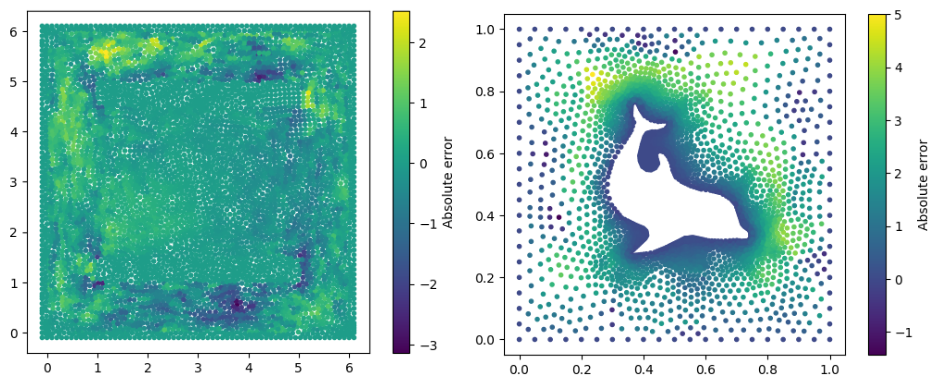
\includegraphics[width = 0.99\linewidth]{Figures/FEM/Errors.png}
    \caption{Absolute Error Plot for the Two complex geometries explored. Left: absolute error for the two conducting bars problem, notice the good math in the zone between the two bars. Right: absolute error for the coaxial dolphin, we have not a very good match on some zones, however we were able to solve this problem with highly complex problem using our algorithm and the solution in reasonable good.}
    \label{fig:Errors}
\end{figure}

\FloatBarrier
\section{A Proof for the General Finite Differences Method}
\label{sec:gfdm_math}
Established FDM discretize a PDE into a (Cartesian) grid then use systems of equations to solve the potential for each element of the mesh. Systems of equations are generated using finite differences between points of the grid.

As an example, an established Cartesian finite difference algorithm for Laplace's equation in two dimensions is
\begin{equation}
    V_{i,j} = \frac{1}{4}[ 
    V_{i+1,j} +
    V_{i-1,j} +
    V_{i,j+1} +
    V_{i,j-1}]
\end{equation}
where $V_{i,j}$, is the current estimation of potential at a Cartesian grid point $(i,j)$ \cite{Landau2015}. The algorithm estimates the potential for a point using the average potentials of its neighbors and avoids solving linear equations instead using an iterative improvement process.

The method is computationally efficient for boundary geometries that satisfy a Cartesian grid. If the problem is not modelled well by a Cartesian coordinate system, slow convergence may occur with decreasing grid spacing. The method then becomes computationally inefficient if a highly precise solution is needed.

We present a generalization of the finite difference method for a general mesh. This mesh we implement as a discretized graph data structure. Each node of the mesh still has its potential informed by neighbors, but the member and its neighbors are not fixed to any particular regular coordinate system. A node may have an arbitrary number of neighbors, and a node may have arbitrary horizontal and vertical offsets with respect to any neighbor.

We desire for every node on the mesh,
\begin{equation}
    \nabla^2 V_i = 0
\end{equation}
where $V_i$ is the potential at some indexed node, $i$. We approximate the horizontal second partial derivative of the potential with respect to one neighbor, $j$, using a quadratic approximation
\begin{equation}
    \frac{\partial^2 V_i}{\partial x^2} \bigg\vert_j \approx
    \frac{1}{2}\frac{V_j - V_i}{(x_j-x_i)^2}
\end{equation}
The same form is used for the vertical term. Combining these quotient approximations,
\begin{equation}
    \nabla^2 V_i \vert_j = \frac{\partial^2 V_i}{\partial x^2} \bigg\vert_j + \frac{\partial^2 V_i}{\partial y^2} \bigg\vert_j \approx
    \frac{V_j - V_i}{2}\bigg[\frac{1}{(x_j - x_i)^2} + \frac{1}{(y_j - y_i)^2}\bigg]
\end{equation}
The inverse square positional terms are constants of the mesh and are easily computed. For brevity, define constants
\begin{equation}
    \gamma_{i,j} = \frac{1}{2}\bigg[\frac{1}{(x_j - x_i)^2} + \frac{1}{(y_j - y_i)^2}\bigg]
\end{equation}
So we approximate the Laplacian of the potential for some node, $i$ with respect to only one neighbor, $j$, as
\begin{equation}
    \nabla^2 V_i \vert_j \approx (V_j - V_i)\gamma_{i,j}
\end{equation}

This approximation is intended to be carried out by many neighbors surrounding the node, $i$. To inform node $i$ of its potential from an arbitrary number of neighbors, we average over the neighbors of $i$ using
\begin{equation}
    \nabla^2 V_i \approx \frac{1}{|n(i)|} \sum_{j \in n(i)} \nabla^2 V_i \vert_j \approx \frac{1}{|n(i)|} \sum_{j \in n(i)} \gamma_{i,j}(V_j - V_i)
\end{equation}
where $n(i)$ is the set of neighbor nodes for a node, $i$, and $|n(i)|$ is the size of the set. We now average informed estimations from individual neighbors over all neighbors of $i$. Because we are solving Laplace's equation, this average equals zero for all $i$. For the special case of Poisson's Equation, we can discard the coefficient involving the size of the neighbor set.
\begin{equation}
    0 \approx \sum_{j \in n(i)} \gamma_{i,j} (V_i - V_j) =
    V_i \sum_{k \in n(i)} \gamma_{i,k} - \sum_{j \in n(i)} \gamma_{i,j} V_j
\end{equation}
Rearranging the expression,
\begin{equation}
    0 \approx -V_i + \frac
    {\sum_{j \in n(i)} \gamma_{i,j} V_j }
    {\sum_{k \in n(i)} \gamma_{i,k}}
    \label{eq:gfdm_proof_final_per_node}
\end{equation}

We want to express the problem as an $m \times m$ where $m$ is the number of nodes in the mesh:
\begin{equation}
    \alpha_i = \sum_j c_{i,j} V_j \;\;\;\;\;\; \forall i
    \label{eq:gfdm_matrix_multiplication}
\end{equation}
where $c_{i,j}$ are the elements of an $m \times m$ matrix expressing the linear system of equations. $\alpha_i$ is an expression of possible Dirichlet boundary conditions. We construct $c_{i,j}$ and $\alpha_i$ to satisfy Equation \ref{eq:gfdm_proof_final_per_node} so that
\begin{equation}
c_{i,j} = \cases{
  -1 & $i = j$, $i$ is not a boundary \cr
  0 & $i \not= j$, $i$ is not a boundary, $j \not\in n(i)$ \cr
  $\gamma_{i,j}(\sum_{k \in n(i)} \gamma_{i,k})^{-1}$ & $i \not= j$, $i$ is not a boundary, $ j \in n(i)$ \cr
  1 & $ i = j $, $i$ is a boundary
  }
  \label{eq:gfdm_matrix_elements}
\end{equation}
and
\begin{equation}
\alpha_i = \cases{
  $\phi_i$ & $i$ is a boundary \cr
  0     & $i$ is not a boundary
}
\end{equation}
where $\phi_i$ is the known potential assigned as a Dirichlet boundary condition to the node $i$. When constructed this way, matrix multiplication is naturally performed so the Dirichlet condition for a boundary node becomes
\begin{equation}
    V_i = \phi_i
\end{equation}

The general method, then, is to iterate once through nodes in a mesh and build the matrix, $c_{i,j}$. We then pass the system to a linear algebra package and extract a solution for the potential at every node.

\begin{comment}
\section{Weak Form of the Poisson Equation}
Now, the algorithm to transform Poisson's equation into its weak form consists of multiplying it by a function $v$, which is called the test function. We ask that $v$ be a continuous function and that meet the condition $v=0$ on the boundary $\Gamma$, which is split into $\Gamma_D$ for the Dirichlet conditions and $\Gamma_N$ for the Neumann conditions. The result is integrated over the domain on which the original problem is defined, in this case $\Omega$, that is
\begin{equation}
     -\int_{\Omega}d\Omega(\nabla^2u) v = \int_{\Omega}d\Omega fv.
\end{equation}
Now we integrate by parts and use the following fact
\begin{equation}
     \int_{\Omega}d\Omega (\nabla^2u)v = -\int_{\Omega}d\Omega(\nabla u)\cdot (\nabla v) + \int_{\partial\Omega}ds( \partial_nu)v,
\end{equation}
where $\partial_nu = \nabla u \cdot n$ is the derivative of $u$ on the boundary in the outward normal direction. $\partial \Omega$ is used to denote the boundary of $\Omega$ and $ds$ is the differential element of the boundary. So we have the following problem
\begin{equation}
     \int_{\Omega}d\Omega\nabla u\cdot \nabla v - \int_{\partial\Omega}ds(\partial_nu)v = \int_{\Omega}d\Omega fv.
\end{equation}
However, the boundary is formed by the union of the sets $\Gamma_D$ and $\Gamma_N$, that is
\begin{equation}
     \int_{\partial\Omega}ds(\partial_nu)v = \int_{\Gamma_D}ds(\partial_nu)v + \int_{\Gamma_N}ds(\partial_nu)v,
\end{equation}
However, by condition (3.35), we have that the previous equation results in
\begin{equation}
     \int_{\partial\Omega}ds(\partial_nu)v = \int_{\Gamma_N}ds(\partial_nu)v,
\end{equation}
but, using condition (3.34), we have to
\begin{equation}
     \int_{\partial\Omega}ds(\partial_nu)v = -\int_{\Gamma_N}dsgv.
\end{equation}
With which, we finally arrive at the weak formulation of the Poisson equation, that is
\begin{equation}
     \int_{\Omega}d\Omega\nabla u\cdot \nabla v - \int_{\Gamma_N}dsgv = \int_{\Omega}d\Omega fv.
\end{equation}
Which written in a precise mathematical way is: find $u\in V$, such that
\begin{equation}
     \int_{\Omega}d\Omega\nabla u\cdot \nabla v= \int_{\Omega}d\Omega fv - \int_{\Gamma_N}dsgv ; \ \ \ \forall v\in \hat{V}.
\end{equation}
In this form, the problem and thus the solution is in a continuous form. The FEM finds an approximate solution to this form by replacing the function space $V$ and $\hat{V}$ with discrete spaces $V_h \subset V$ and $\hat{V}_h \subset \hat{V}$. Therefore the problem becomes: find $u_h \in V_h \subset V$, such that
\begin{equation}
    \int_{\Omega}d\Omega\nabla u_h \cdot \nabla v= \int_{\Omega}d\Omega fv - \int_{\Gamma_N}dsgv ; \ \ \ \forall v\in \hat{V}_h \subset \hat{V}.
\end{equation}

\end{comment}

\end{document}
